% !TEX root = main.tex
\label{ch:campaigns}
Computational campaigns enact an execution to achieve a computation objective under given requirements and constraints.
The computational objective is a set of values selected by the user for a set of metrics.
Some of these metrics are time to completion and throughput.
Furthermore, the objective can be represented as an objective function.
Requirements describe the minimum amount and type of resources needed to execute each workflow of the campaign, while the constrains are the conditions that bound the the execution, such as resource availability, resource capacity or costs.

The objective of a campaign can be translated to a computational objective function that would either minimize or maximize a metric.
Among the many metrics that could be considered, the most common one is the total time taken by a campaign to execute, also known as makespan.
An execution plan of a campaign is a mapping between workflows and resource to execute upon.
Calculating the makespan of a campaign means finding an execution plan that satisfies the computational objective function.

A computational campaign execute on several HPC resources.
These resources are heterogeneous as they offer different type of resources.
One aspect of this heterogeneity is the performance each HPC resources has in terms of Peta-Flops.
In addition, these resources are dynamic as their availability and performance can change over time.

Users have deep knowledge of their workflows and their requirements when they prototype them.
As a result, they may not know accurately the total number of operations of each workflow that comprise their campaign.
This, in turn, makes it even harder to derive an execution plan that will satisfy the objective of the campaign.

We use a campaign from a campaign from a polar science use case to evaluate three classes of planning algorithms.
These classes differ on how they approach the planning problem and in the amount of knowledge they produce to derive a plan.
We experimentally measure and characterize the performance of these classes.

The chapter offers the following contributions:
\begin{inparaenum}[i)]
    \item an experiment-based methodology to compare planning algorithms performance that does not depend on the considered use case and computing framework;
    \item a conceptual framework for selecting planning algorithms based on the algorithm, campaign and resources characteristics
\end{inparaenum}

The chapter is organized as follows: \S~\ref{sec:makespan_calc} discusses the calculation of the makespan of a campaign given the set of assumptions of this work.
Section \S~\ref{sec:algo} discusses three selected makespan calculation algorithms and \S~\ref{sec:algo_perf_comp} compares their performance, i.e the derived makespan.
Finally, section \S~\ref{sec:cf_algo_sel} presents a conceptual framework that will allow users to best select a planning algorithm.

% -------------------------------------------------------------------
\section{Calculating the Makespan of a Campaign}
\label{sec:makespan_calc}
The way workflows of a given campaign are mapped to resources can affect the makespan calculation. 
Figure~\ref{fig:example_makespan} shows an example of a campaign with workflows of different size and execution times, and the makespans that two different mappings produce.
The makespan of the campaign on the left sub~-figure is $20$, while on the right it is $16$.
In addition, the size of the workflows, i.e., the number of resources they require, becomes relevant and resources may be underutilized, as shown in Figure~\ref{fig:example_makespan}.

\begin{figure*}[ht!]
    \centering
    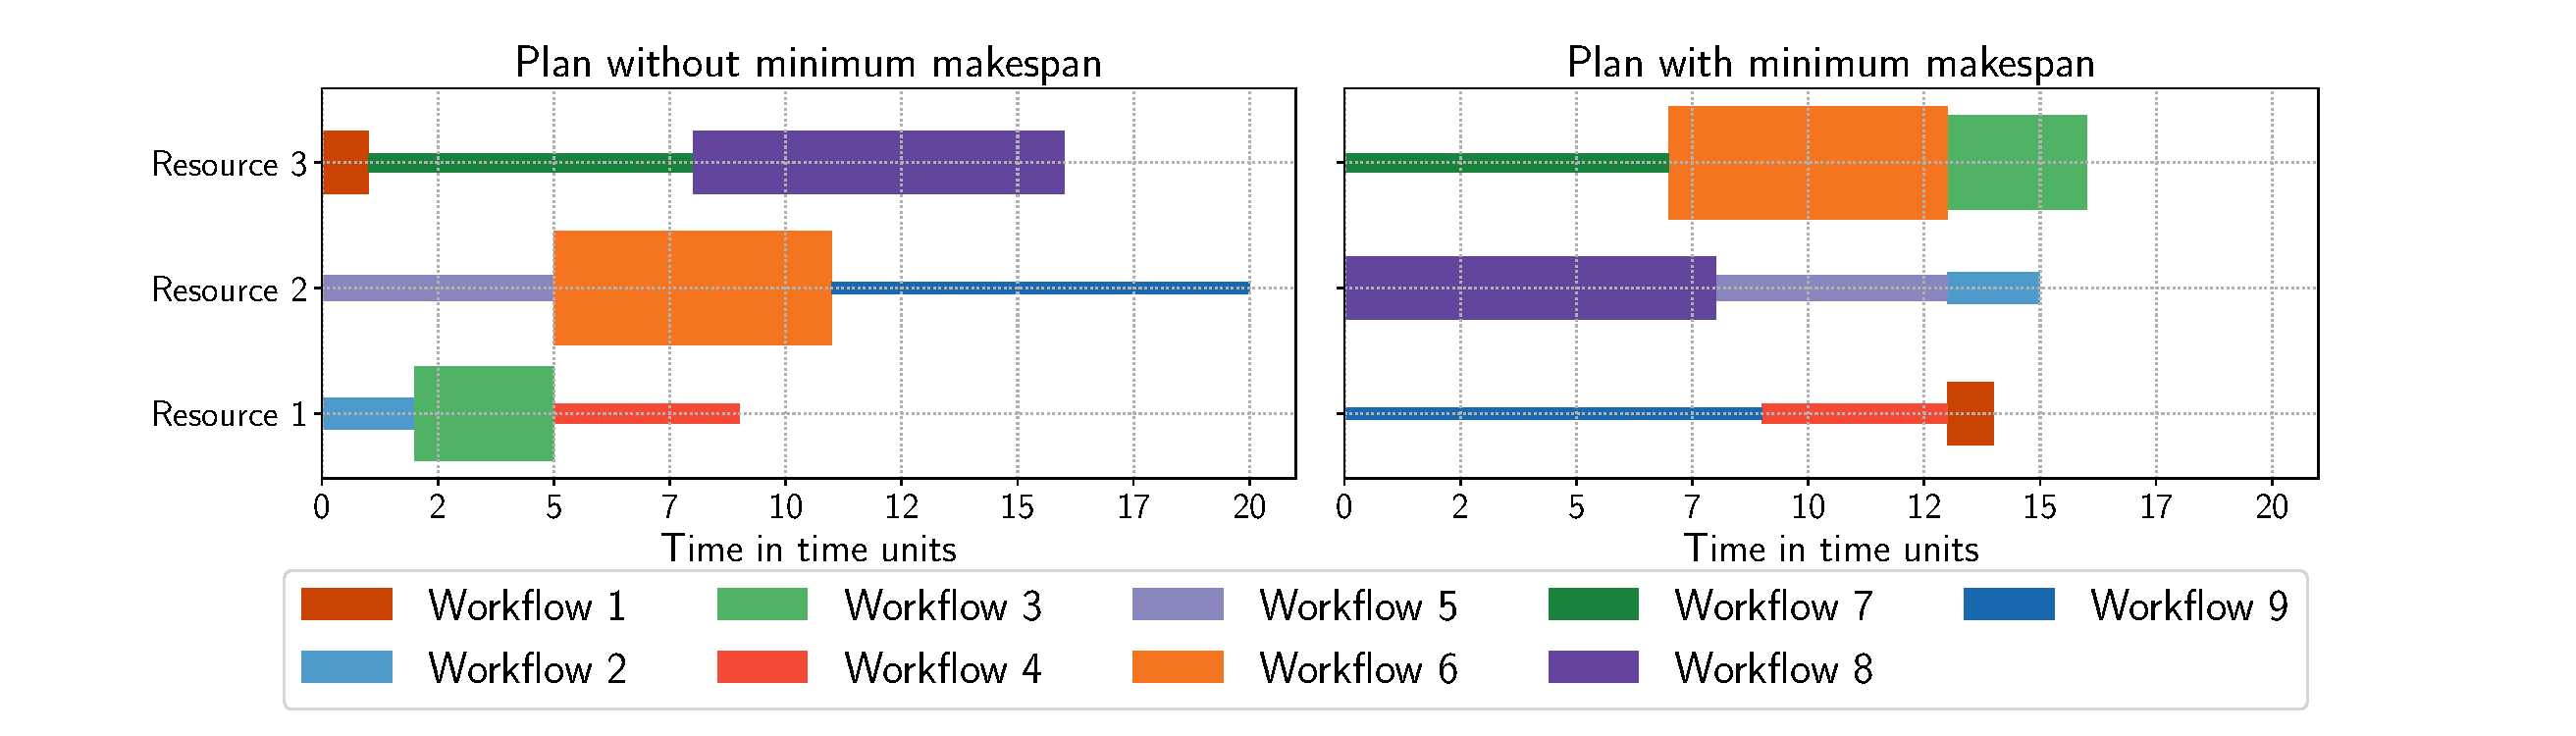
\includegraphics[width=.99\textwidth]{figures/campaign/plan_comp.pdf}
    \caption{Comparison of different campaign execution plans. Based on workflow mapping on resources makespan and resource utilization is different.}\label{fig:example_makespan}
\end{figure*}

We are making a set of assumptions which we do not relax during the analysis of a model that calculates the makespan of a campaign.
These are:
\begin{inparaenum}[(1)]
    \item a workflow is an atomic unit and cannot be decomposed;
    \item workflow resource request is sufficient to execute the workflow;
    \item a resource is an aggregate of computing capabilities;
    \item every workflow of a given campaign can be executed on the given resources;
    \item random resource selection is based on a uniform distribution;
    \item only one workflow can be executed on a resource at any point in time; and
    \item workflows can be homogeneous or heterogeneous in space---maximum number of resources they need, and time---the amount of time they are executing.
\end{inparaenum}

We denote a computational campaign as $C = [w_{i}: 1 \leq i \leq N_{C}]$, where $w_{i}$ is a workflow and $N_{C}$ is the total number of workflows, $R = [ r_{j}: 1 \leq j \leq N_{R}]$ is a set of available resources, where $r_{j}$ is a resource and $N_{R}$ is the total number of available resources, and $ M(C,R) = [(w_i, r_j): 1 \leq i \leq N_{C}, r_j \in R] $ is a mapping function of workflows onto resources.
In addition, we denote the execution time of a workflow as $Tx_{w_{i}}$, the makespan of campaign $C$ as $TTX_{C}$, and the makespan of campaign $C$ for a given mapping function $ M $ as $TTX_{C}(M)$.
Assumption~\#3 allows to abstract the resource implementation details, as workflows can be executed on different resources such as HPCs, Clouds, pilots and more. 
%Lastly, we will assume initially homogeneous resources as it simplifies the formalization of the problem.

With a single resource, i.e., $N_{R} = 1$, the workflows of a campaign will be executed sequentially, regardless the execution order or if the workflows are homogeneous or heterogeneous.
As a result the makespan of the campaign is:
\begin{equation}
   TTX_{C} = \sum_{i=1}^{N_{C}}Tx_{w_{i}} 
\end{equation}

With multiple resources, i.e., $1 < N_{R} < N_{C}$, the workflows of a campaign can be executed concurrently.
With homogeneous resources, this is semantically equivalent to executing on a single resource large enough to allow concurrent workflow execution, where each workflow executes on a resource partition. 
Because of assumptions~\#4 and~\#7, executing homogeneous or heterogeneous in space workflows has the same makespan.
A random mapping of workflows onto resource will have a makespan:
\begin{equation}
   TTX_{C}(Random) \geq \frac{1}{N_{R}}\sum_{i=1}^{N_{C}} Tx_{w_{i}} 
\end{equation}
Given multiple homogeneous resources, when executing workflows that are heterogeneous in time and that can be homogeneous or heterogeneous in space, the makespan of the campaign for a given mapping function $ M $ is:
\begin{equation}
TTX_{C}(M) = \max_{r_{j}\in R}\Big\{\sum_{w_{i}\in M(C,r_{j})}Tx_{w_{i}}\Big\}
\label{eq:makespan}
\end{equation}
Relaxing the assumption that resources are heterogeneous, in the performance they offer, affects the result of the mapping function $ M $.
As a result, Eq.~\ref{eq:makespan} holds in calculating the makespan of the campaign.

Computational campaigns execute to achieve an objective.
We consider as objective the total time of completion of the campaign.
As a result, the objective function of a plan is translating in minimizing the value of eq;~\ref{eq:makespan}.
As objective function is:
\begin{equation}
    \min(\max_{r_{j}\in R}\Big\{\sum_{w_{i}\in M(C,r_{j})}Tx_{w_{i}}\Big\})
\end{equation}
In the next section, we discuss a set of algorithms that try to satisfy this objective function.

% -------------------------------------------------------------------
\section{Planning Algorithms}
\label{sec:algo}

There is a plethora of methods and algorithms to calculate and optimize the makespan of a workflow~\cite{lu2019review}, including queuing networks~\cite{yao2019throughput,bao2019performance}, domain specific languages~\cite{carothers2017durango,maheshwari2016workflow}, and machine learning~\cite{witt2019predictive,pumma2017runtime}.
From this plethora of selections, we selected to investigate three algorithms, each one representative of a larger family of algorithms.
These are Heterogeneous Earlier Finish Time algorithm (HEFT)~\cite{topcuoglu2002performance}, a genetic algorithm~\cite{page2005algorithm} and a simple heuristic algorithm.

The following sections present the selected algorithms in more detail.
In addition to the algorithmic details, we discuss the knowledge and the information each algorithm produces to derive a plan.
A summary of the algorithms characteristics are shown in Table~\ref{tab:sched_algo}.

\begin{table}[t]
    \centering
    \scriptsize
    \begin{tabular}{@{}ccccc@{}}
        \toprule
        &\textbf{HEFT}     &\textbf{Genetic Algorithm} &\textbf{L2FF} & \textbf{Random} \\
        \midrule
        Decision Policy   &Deterministic &Convergence Criteria &Deterministic& Deterministic\\
        Initial State    &Blank &Semi-random &Blank & Blank\\
        \midrule
        \multicolumn{5}{l}{\textbf{Initial Knowledge}}\\\midrule
        Workflow Operations &Yes & Yes & Yes & No\\
        Resource Performance &Yes &Yes &Yes & No\\
        \midrule
        Produced Knowledge& Resource availability& Resource availability&None&None\\
        \bottomrule
    \end{tabular}
    \caption{Basic characteristics of selected planning algorithms.\label{tab:sched_algo}}
\end{table}

% -------------------------------------------------------------------
\subsection{Heterogeneous Earlier Finish Time (HEFT) algorithm}
\label{algo:heft}
List scheduling algorithms represent a general family of heuristic based scheduling algorithms to schedule workflows described as direct acyclic graphs~\cite{dong2006scheduling,list_sched_wiki}. 
These algorithms assign priorities to tasks based on a heuristic and order them non-increasingly based on the derived priorities.
Then, this list is traversed and tasks are assigned to resources.
HEFT is a classic example of this type of algorithms~\cite{dong2006scheduling}.

HEFT is an offline scheduling algorithm which calculates the makespan of a workflow on heterogeneous resources, in terms of performance.
HEFT has been implemented as part of the planning capabilities in Pegasus~\cite{deelman2015pegasus} and ASKALON~\cite{fahringer2005askalon} amongst other algorithms.
HEFT has been shown to provide better performance in terms of makespan minimization compared to other mapping algorithms~\cite{topcuoglu2002performance,fahringer2005askalon,canon2008comparative}. 

HEFT makes two important assumptions when used on multiple workflows, i.e., a campaign: 
\begin{inparaenum}[(1)] 
    \item any task in a workflow can be executed on all available resources; and 
    \item all resources are always available.
\end{inparaenum}
HEFT is mainly used to derive an execution plan for workflows, i.e., the execution order and resource placement of the tasks that comprise the workflow.
HEFT uses a matrix to represent execution time of tasks on resources, assigning tasks to the resource that minimizes the finish time of the task, and has complexity proportional to the number of dependencies between tasks and the number of resources offered. 
Because we are interested in campaigns, our HEFT extension will provide an execution plan based on workflows as atomic units instead of tasks.
Furthermore, there has been some initial research to extend HEFT to resources that provide CPU and GPUs~\cite{shetti2013optimization}, as well as a HEFT extension on dynamic resources~\cite{dong2007pfas}. 
Algorithm~\ref{alg:heft} shows HEFT for placing independent heterogeneous workflows on heterogeneous resources.

\begin{algorithm}[ht]
    \caption{Heterogeneous Earliest Finish Time (HEFT) algorithm}
    \label{alg:heft}
    \begin{algorithmic}[1]
        \Procedure{HEFT}{$W$,$R$}\Comment{$W$ and $R$ are a set of workflow and resources respectively}
        \State \texttt{Calculate the computation cost $w_{tx}^{ij}$ of each workflow for all resources}
        \State \texttt{Assign $rank_i = \overline{w_{i}} = \nicefrac{\sum_{j=1}^{|R|}w_{tx}^{ij}}{|R|}$}
        \State \texttt{Sort workflows by non-increasing order of $rank_i$}
        \While{unscheduled workflows}
        \State \texttt{Select the first workflow $\tilde{w}$ from the sorted list}
        \For{$\forall r_{j}$ in $R$}
        \State\texttt{Compute earliest finish time for $\tilde{w}$ on $r_{j}$, $eft_{\tilde{w},r_j}$ }
        \EndFor
        \State \texttt{Assign  $\tilde{w}$ on $r_k$ with $\min{(eft_{\tilde{w},r_j})}$}
        \EndWhile
        \EndProcedure
    \end{algorithmic}
\end{algorithm}

As mentioned above HEFT makes the assumption that all resources are always available and static.
Based on this assumption, HEFT makes the implicit assumption that resources are available based on the times it internally computes.
As a result, it has no external knowledge or representation of when a resource becomes available.
HPC resources may become unavailable for multiple reasons, including but not limited to maintenance, a random failure, executing a workflows over the expected time., etc.
In order to be able to utilize HEFT for dynamic resources, we had to extend Algorithm~\ref{alg:heft} to take as input the time that a resource is initially available.
This input can be represented as a dictionary where the keys are the available resources and the values are the time a resource becomes available.
The extended algorithm is shown in Algorithm~\ref{alg:ext_heft}.
Although the extension may be small, it is crucial to allow to reuse HEFT based on the state of the execution at a given point in time.

\begin{algorithm}[ht]
    \caption{Extended Heterogeneous Earliest Finish Time (EHEFT) algorithm}
    \label{alg:ext_heft}
    \begin{algorithmic}[1]
        \Procedure{EHEFT}{$W$, $R$, $T$}\Comment{$W$ and $R$ are a set of workflow and resources respectively. $T$ is a dictionary of when a resource becomes available.}
        \State \texttt{Calculate the computation cost $w_{tx}^{ij}$ of each workflow for all resources}
        \State \texttt{Assign $rank_i = \overline{w_{i}} = \nicefrac{\sum_{j=1}^{|R|}w_{tx}^{ij}}{|R|}$}
        \State \texttt{Sort workflows by non-increasing order of $rank_i$}
        \While{unscheduled workflows}
        \State \texttt{Select the first workflow $\tilde{w}$ from the sorted list}
        \For{$\forall r_{j}$ in $R$}
        \State\texttt{Compute earliest finish time for $\tilde{w}$ on $r_{j}$ based on $T(r_j)$, $eft_{\tilde{w},r_j}$ }
        \EndFor
        \State \texttt{Assign  $\tilde{w}$ on $r_k$ with $\min{(eft_{\tilde{w},r_j})}$}
        \EndWhile
        \EndProcedure
    \end{algorithmic}
\end{algorithm}

% -------------------------------------------------------------------
\subsection{Genetic Algorithm}
\label{algo:gen}
Genetic algorithms are represent another family of algorithms that are been used to minimize the makespan of an execution~\cite{dong2006scheduling}.
Genetic algorithms are evolving to the final answer as they iterate and improve possible answers.
In general, genetic algorithms are working based on the following procedure:
\begin{inparaenum}[(i)]
    \item create an initial population, where the population is a set of chromosomes. 
          Chromosomes, in the context of planning the execution workflows on resources, is a potential placement of workflows on resources;
    \item evaluate the chromosomes based on a fitness value, which represents the makespan on the campaign;
    \item reproduce by selecting chromosomes, either randomly or based on their fitness value, and generate a new set of chromosomes (called children);
    \item mutate randomly, where randomly selected workflows from a random chromosome are reassigned to resources; and
    \item re-evaluate chromosomes in the population to check convergence.
\end{inparaenum}

The selected genetic algorithm~\cite{page2005algorithm} is developed to support the placement of independent task on heterogeneous resources.
It assumes that all tasks can be executed on all available resources, are independent and indivisible.
These assumptions are in accordance with the assumptions made for workflows in a campaign.
As a result, this algorithm can be extended to support scientific campaigns.
The pseudocode of this algorithm is shown in Algorithm~\ref{alg:gen_algo}.

\begin{algorithm}[ht]
    \caption{Genetic Algorithm}
    \label{alg:gen_algo}
    \begin{algorithmic}[1]
        \Procedure{GA}{$W$, $R$, $T$}\Comment{$W$ and $R$ are a set of workflow and resources respectively. $T$ is a dictionary of when a resource becomes available.}
        \State \texttt{Initaliaze population}
        \While{Conergence Criteria not met and \#Gen $<$ Total\_Generations}
        \State{Selection}
        \State{Reproduce}
        \State{Randomly mutate}
        \State{Balance}
        \EndWhile
        \EndProcedure
    \end{algorithmic}
\end{algorithm}

The chromosomes of the initial population are constructed semi-random.
Specifically, a specific percentage of the workflows are assigned randomly to resources, where the assignment is drawn by uniform distribution.
The rest of the workflows are assigned based on an earlier finish time (EFT) heuristic, similar to the one used by HEFT.
The population size is relatively small to 20 chromosomes, i.e., potential plans, called micro-GA.
Micro-GA reduces the computational load of the genetic algorithm, while it does not significantly impact the final result~\cite{zomaya2001observations}.

Selection of the chromosomes to reproduce is based on a fitness function, which calculates the relative distance from a theoretical optimal processing time.
Each chromosome is assigned a fitness value, which then defines the probability of a chromosome to be selected.
Reproduction uses cyclic rotation to generate the new population members.
Mutation randomly selects an individual from the population and randomly swaps workflows.
Finally, a rebalancing heuristic tries to rebalance and create fitter individuals in the population.

We extend this algorithm in the population initialization to support replanning..
The initialization method takes into account the times resources will be available during for the EFT heuristic.
Another point of extension would be the fitness function.
However, the fitness function of the selected algorithm~\cite{page2005algorithm} already takes into account the previous load of a resource, which is the time a resource is available.

% -------------------------------------------------------------------
\subsection{Longest to Fastest First Available Resource Algorithm}
\label{algo:l2ff}
The last algorithm places workflows based on the rule largest workflows to fastest resource~\cite{balasubramanian2019programming}.
This algorithm sorts the workflows based on the number of operations and resources based on their performance.
Then it places each workflow on the first fastest available resource.
Algorithm~\ref{alg:l2ff} show the pseudocode for this algorithm.

\begin{algorithm}[ht]
    \caption{Longest to Fastest First (L2FF)}
    \label{alg:l2ff}
    \begin{algorithmic}[1]
        \Procedure{l2ff}{$W$, $R$}\Comment{$W$ and $R$ are a set of workflow and resources respectively.}
        \State \texttt{$W_{sorted}=sort(W)$} 
        \State \texttt{$R_{sorted}=sort(R)$}
        \For{$w$ in $W_{sorted}$}
        \State{Assign $w$ to $r_{k}$ where $k=w_{idx} \mod N_{R}$}
        \EndFor
        \EndProcedure
    \end{algorithmic}
\end{algorithm}

This algorithm does not specify in any way when resources are either becoming or are available.
As a consequence, there is no need to extend it when dynamic resources are used, as long as the resource performance is updated accordingly.

% -------------------------------------------------------------------
\section{Performance Evaluation of Planning Algorithms}
\label{sec:algo_perf_comp}

We executed three experiments to evaluate and analyze the performance of the selected algorithms.
The first experiment measures the makespan of the plans these algorithms in ideal conditions, providing us with information to rank them.
The second experiment measure the sensitivity of the algorithms when resource performance changes over time.
Last, we measure the sensitivity of the algorithms when there is uncertainty in the total number of operations of the workflows.
These sets of experiments provide a methodology to compare planning algorithms and decide which algorithm is more suited based on the campaign computation requirements, i.e. workflow size, resource performance/availability and initial information uncertainty.

As mention before, resources can be homogeneous or heterogeneous and static or dynamic.
They are homogeneous when the performance, in terms of operations per second, is the same between resources, otherwise they are heterogeneous.
Further, static resources are those whose performance does not change over time and dynamic when the resource performance changes over time.

We use four existing HPC resources as the basis for generating heterogeneous resources.
These resources are PSC Bridges, SDSC Comet, TACC Stampede2 and TACC Frontera.
Each resource performance, as published in the resource documentation, defines the mean value of the distribution.
Figure~\ref{fig:heter_res} shows such resources.
As seen from the figure, the resources are distinct  based on their performance.
As a result, the algorithm that utilizes the faster resources more should provide the better makespan.

\begin{figure}[ht!]
    \centering
    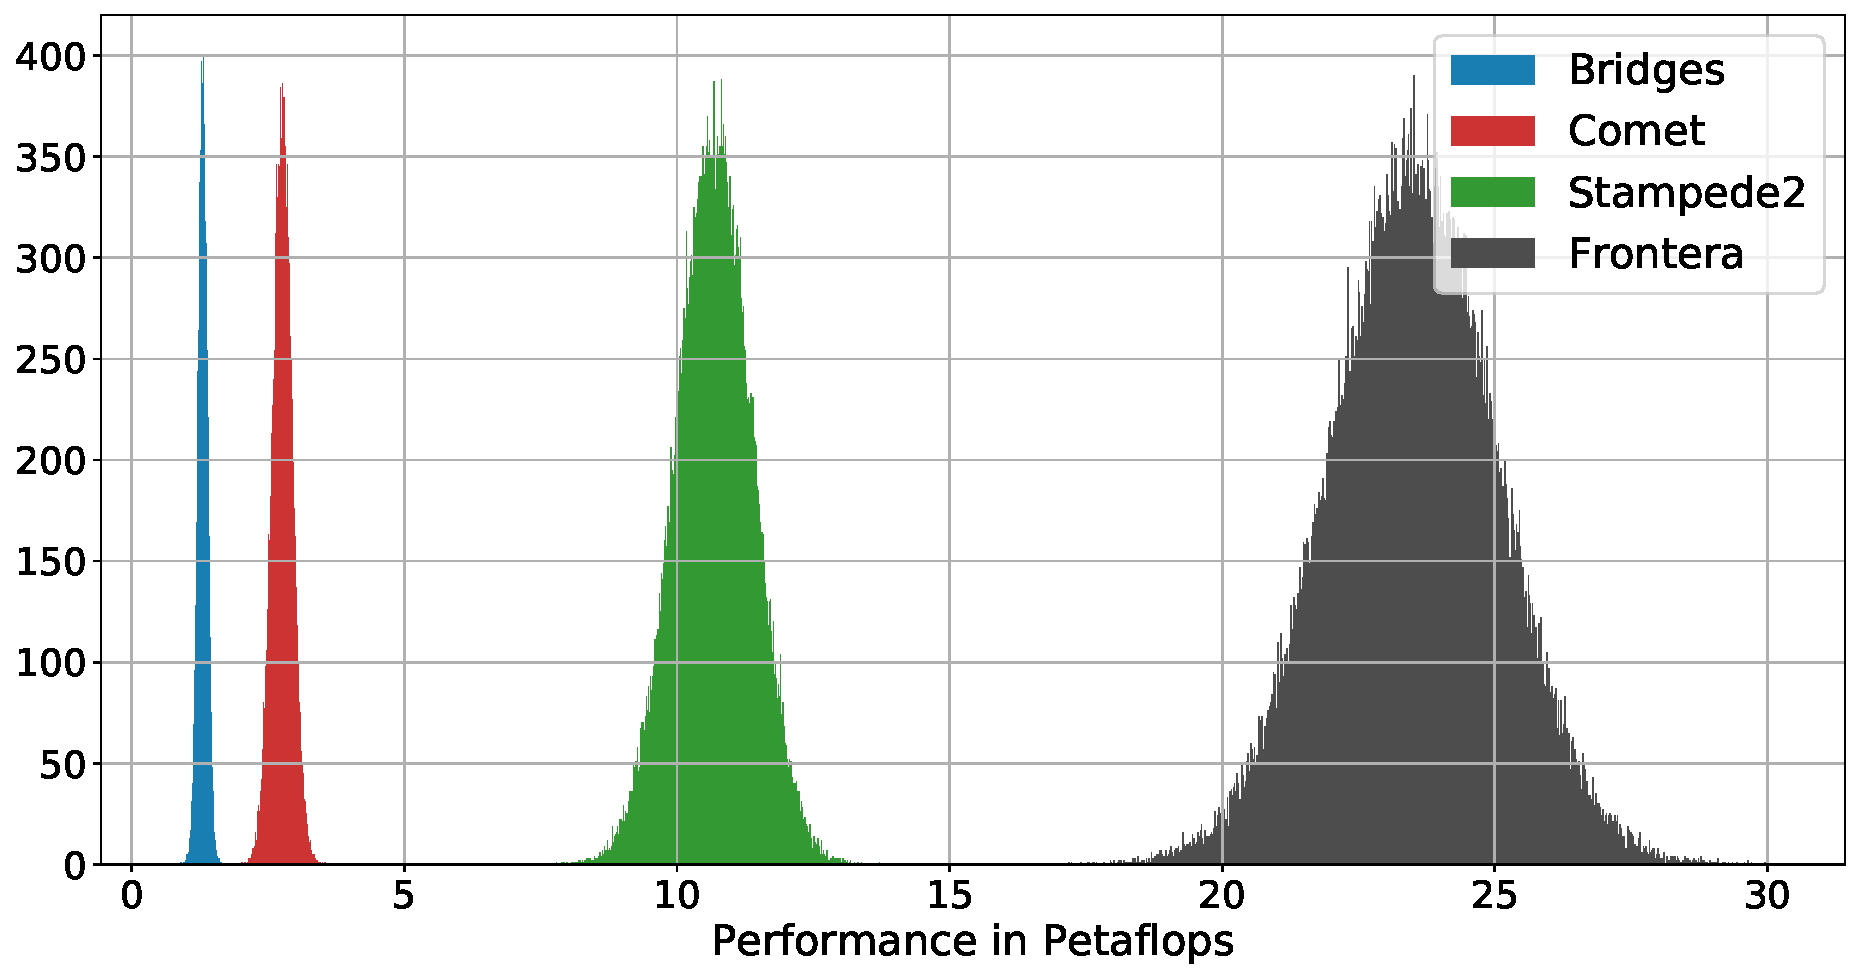
\includegraphics[width=.95\textwidth]{figures/campaign/hetero_res.pdf}
    \caption{Heterogeneous resource distributions.}
    \label{fig:heter_res}
\end{figure}


\subsection{Experiment 1: Measuring makespan on static resources}

In our first experiment, we measure the makespan produced by the selected algorithms for static resources and different configurations of campaign and resource homogeneity/heterogeneity.
In all cases, we either varied the campaign size while keeping the resource number constant or the number of resources while keeping the campaign size constant.

Figure~\ref{fig:st_homog_analysis} shows the results for a campaign with homogeneous workflows and homogeneous resources.
Figure~\ref{fig:StHomoCampaigns_4StHomoResources} compares the makespan produced from HEFT, the genetic algorithm (GA in the figure), L2FF and the Random placement when the campaign size varies from 4 workflows up to 1024.
Figure~\ref{fig:StHomoResources_StHomoCampaigns} makes the same comparison with varying the number of resources for a campaign of 1024 workflows.
The genetic algorithm allows us to select the percentage of the workflows assigned non-randomly for each individual of the population.
We used 0~\% (GA in the figure), 25~\% (GA-25) and 50~\% (GA-50).
In addition, the genetic algorithm stopped evolving its population if it converged, i.e., an individual plan had the ideal makespan, or after 100 iterations and returned the individual in the current population with the best makespan.

\begin{figure}[ht!]
    \centering
    \begin{subfigure}[b]{0.85\textwidth}
        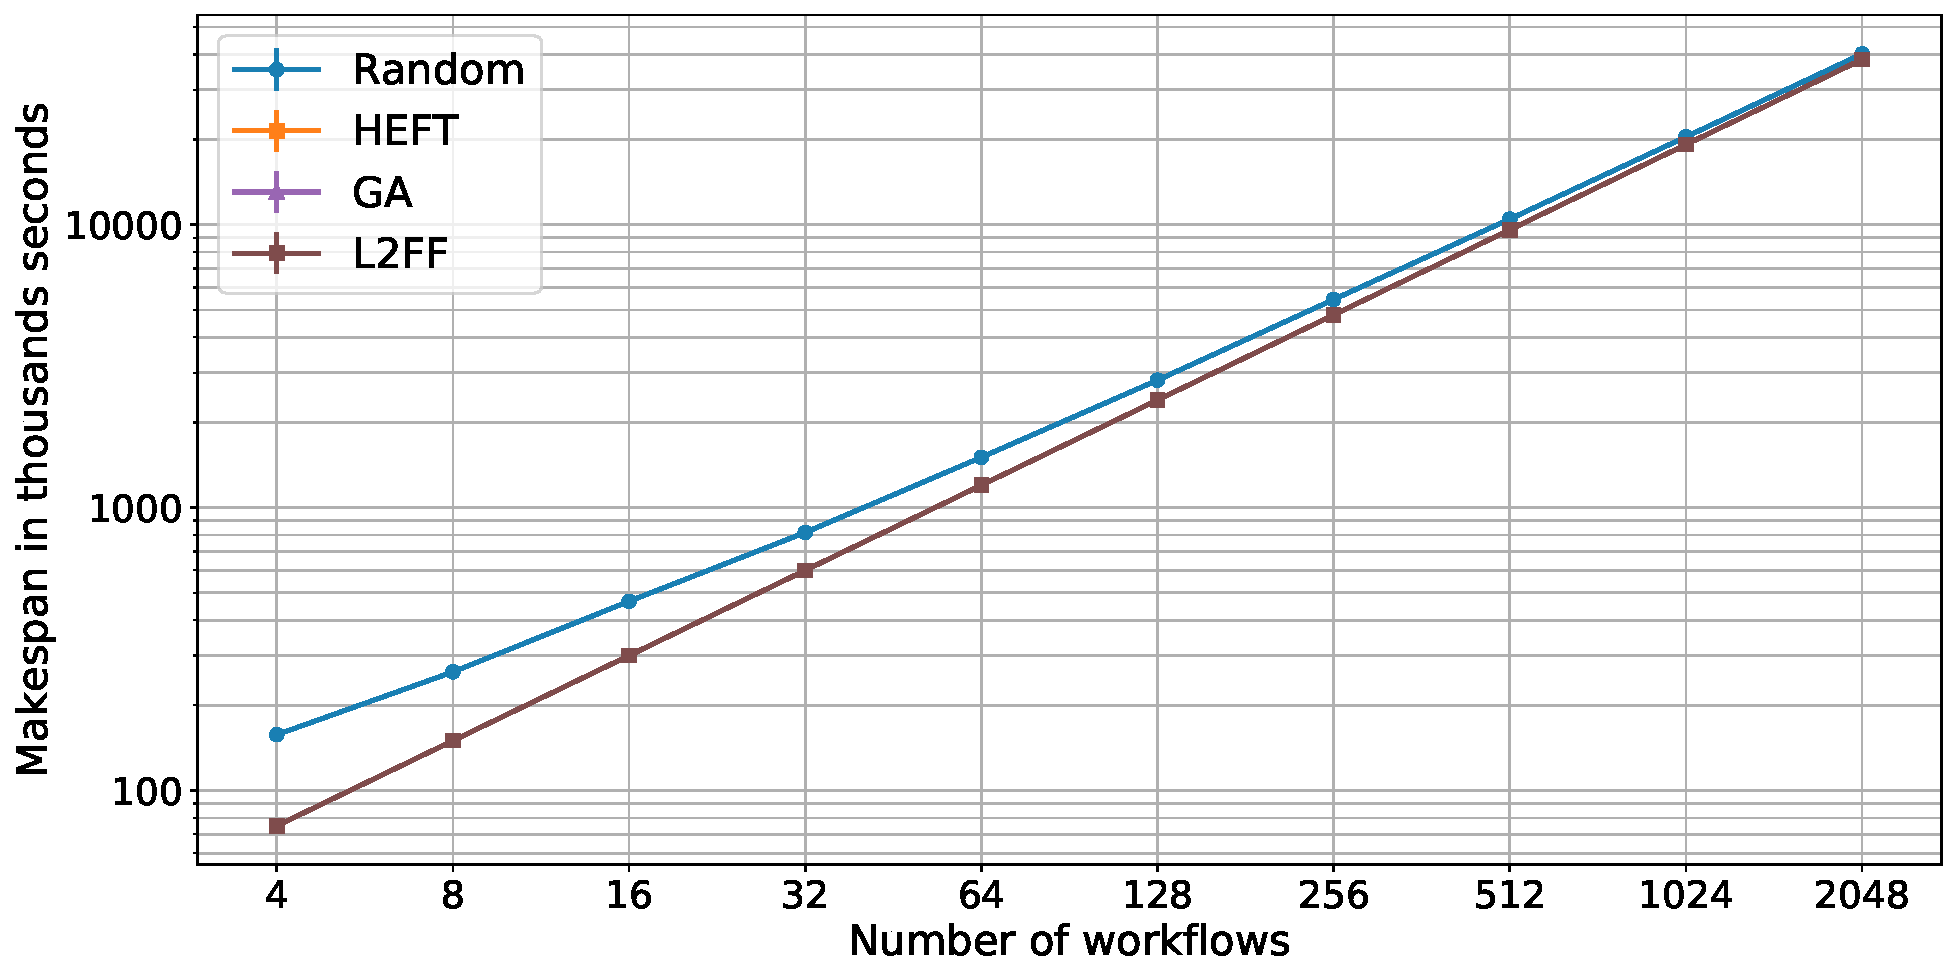
\includegraphics[width=.95\textwidth]{figures/campaign/StHomoCampaigns_4StHomoResources.pdf}
        \caption{}
        \label{fig:StHomoCampaigns_4StHomoResources}
    \end{subfigure}\\
    ~ 
    \begin{subfigure}[b]{0.85\textwidth}
        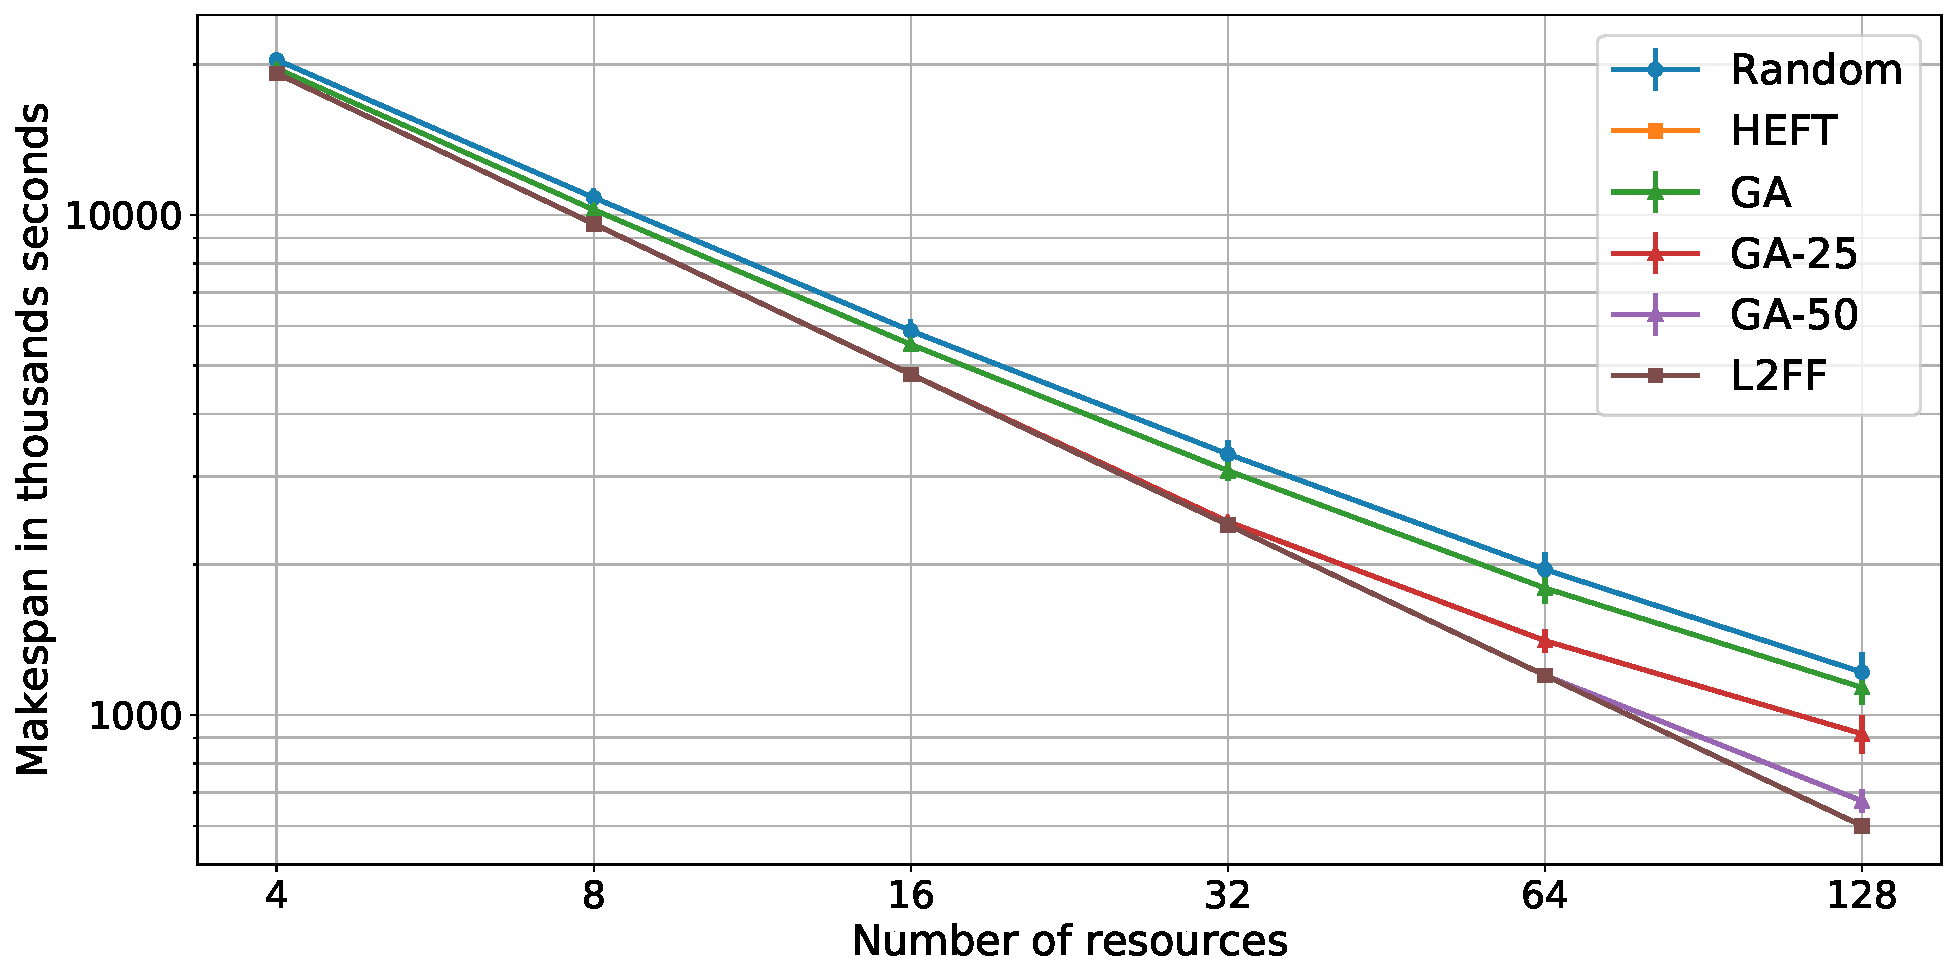
\includegraphics[width=.95\textwidth]{figures/campaign/StHomoResources_StHomoCampaigns.pdf}
        \caption{}
        \label{fig:StHomoResources_StHomoCampaigns}
    \end{subfigure}
    \caption{~\ref{fig:StHomoCampaigns_4StHomoResources} Makespan of increasing number of homogeneous workflows on static homogeneous resources.
    ~\ref{fig:StHomoResources_StHomoCampaigns} Makespan of homogeneous campaign on different number of static homogeneous resources.}
    \label{fig:st_homog_analysis}
\end{figure}

As both figures show, any kind of planning offers better makespan than random placement with a significant margin.
The genetic algorithm that used only random initialization of the population produced the worst out of the three different configurations.
The other two genetic algorithm configuration do not provide significant different performance as the workflows increased, but they show the effect of the random placement when the number of resources increase.
HEFT and L2FF offered the best makespan compared to the genetic algorithm.

\begin{figure*}[ht!]
    \centering
    \begin{subfigure}[b]{0.85\textwidth}
        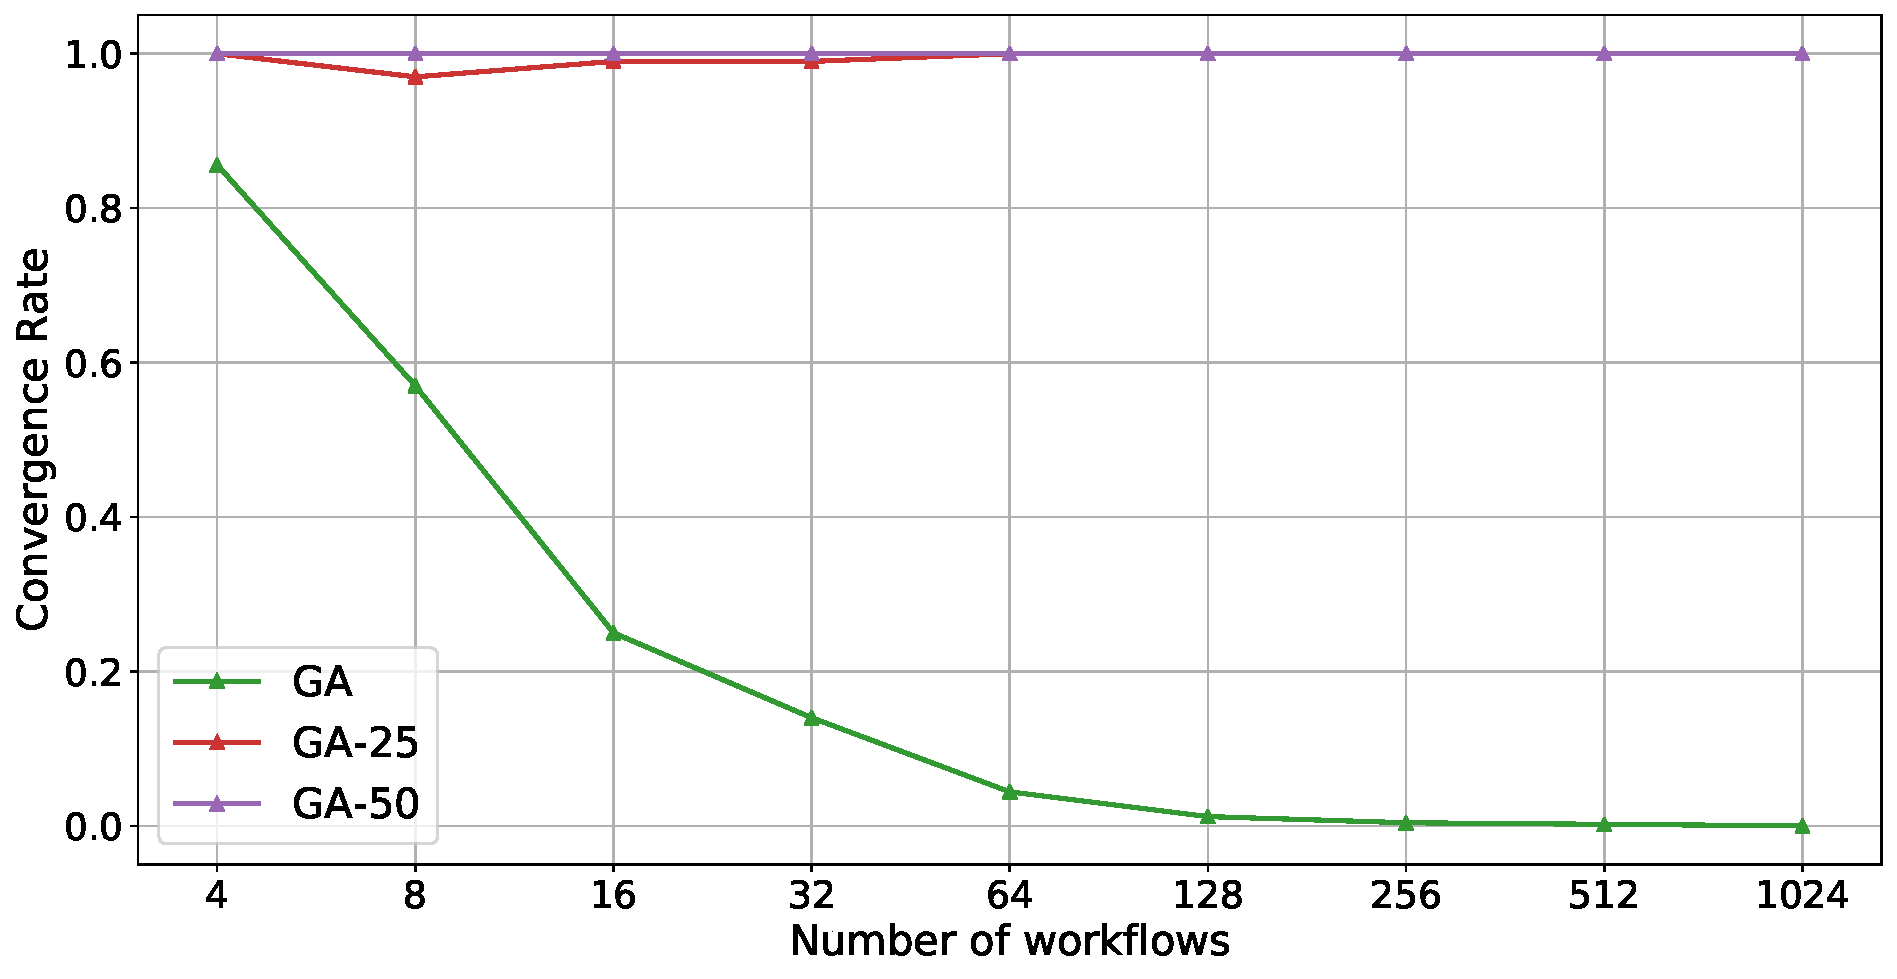
\includegraphics[width=.95\textwidth]{figures/campaign/StHomoCampaigns_4StHomoResourcesGAconv.pdf}
        \caption{}
        \label{fig:ga_conv1}
    \end{subfigure}\\
    ~ 
    \begin{subfigure}[b]{0.85\textwidth}
        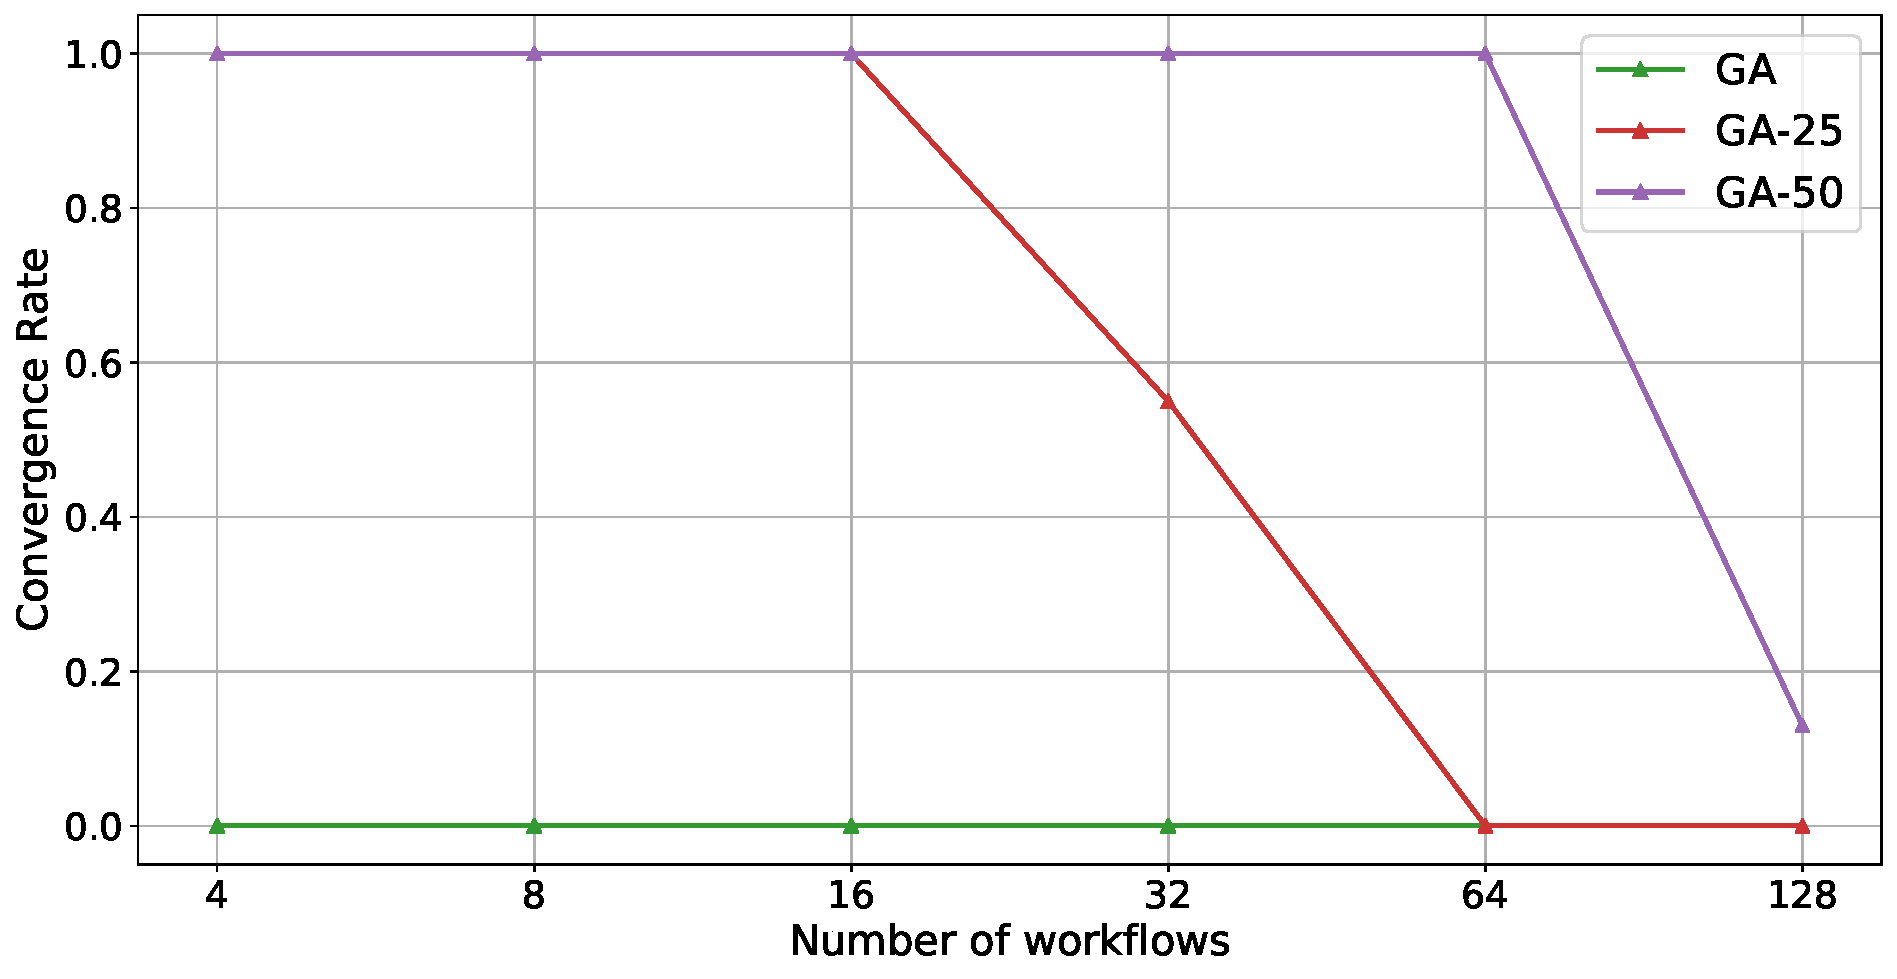
\includegraphics[width=.95\textwidth]{figures/campaign/HomogeResources_StHomogeCampaignsGAconv.pdf}
        \caption{}
        \label{fig:ga_conv2}
    \end{subfigure}
    \caption{Convergence rate of Genetic algorithm for homogeneous campaigns on static homogeneous resources based on random initialization percentage: ~\ref{fig:ga_conv1}) Different campaign sizes on 4 resources;~\ref{fig:ga_conv2}) Campaign with 1024 workflows and different number of resources.}
    \label{fig:conv_rate}
\end{figure*}

The percentage of non-random placement has a significant effect in how able is the algorithm to produce the ideal makespan.
This is supported by figure~\ref{fig:conv_rate} which shows the convergence rate of the three configurations.
The full random initial placement did not produce consistently the ideal makespan even for four workflows and resources.
The other two configurations did consistently produce the ideal makespan when the number of workflows varied.
The small drop in the GA-25 (max of 3 out of 100 iterations) shows that there is still a small probability (max of 3~\%) to not produce the ideal makespan.
In addition, Fig.~\ref{fig:ga_conv2} indicates that as the number of resources increase the performance of the genetic algorithm will drop.
Despite the low convergence of GA-50 on 128 resources the difference from HEFT or L2FF is small which allows us to select this configuration for later experiments.

\begin{figure*}[ht!]
    \centering
    \begin{subfigure}[b]{0.85\textwidth}
        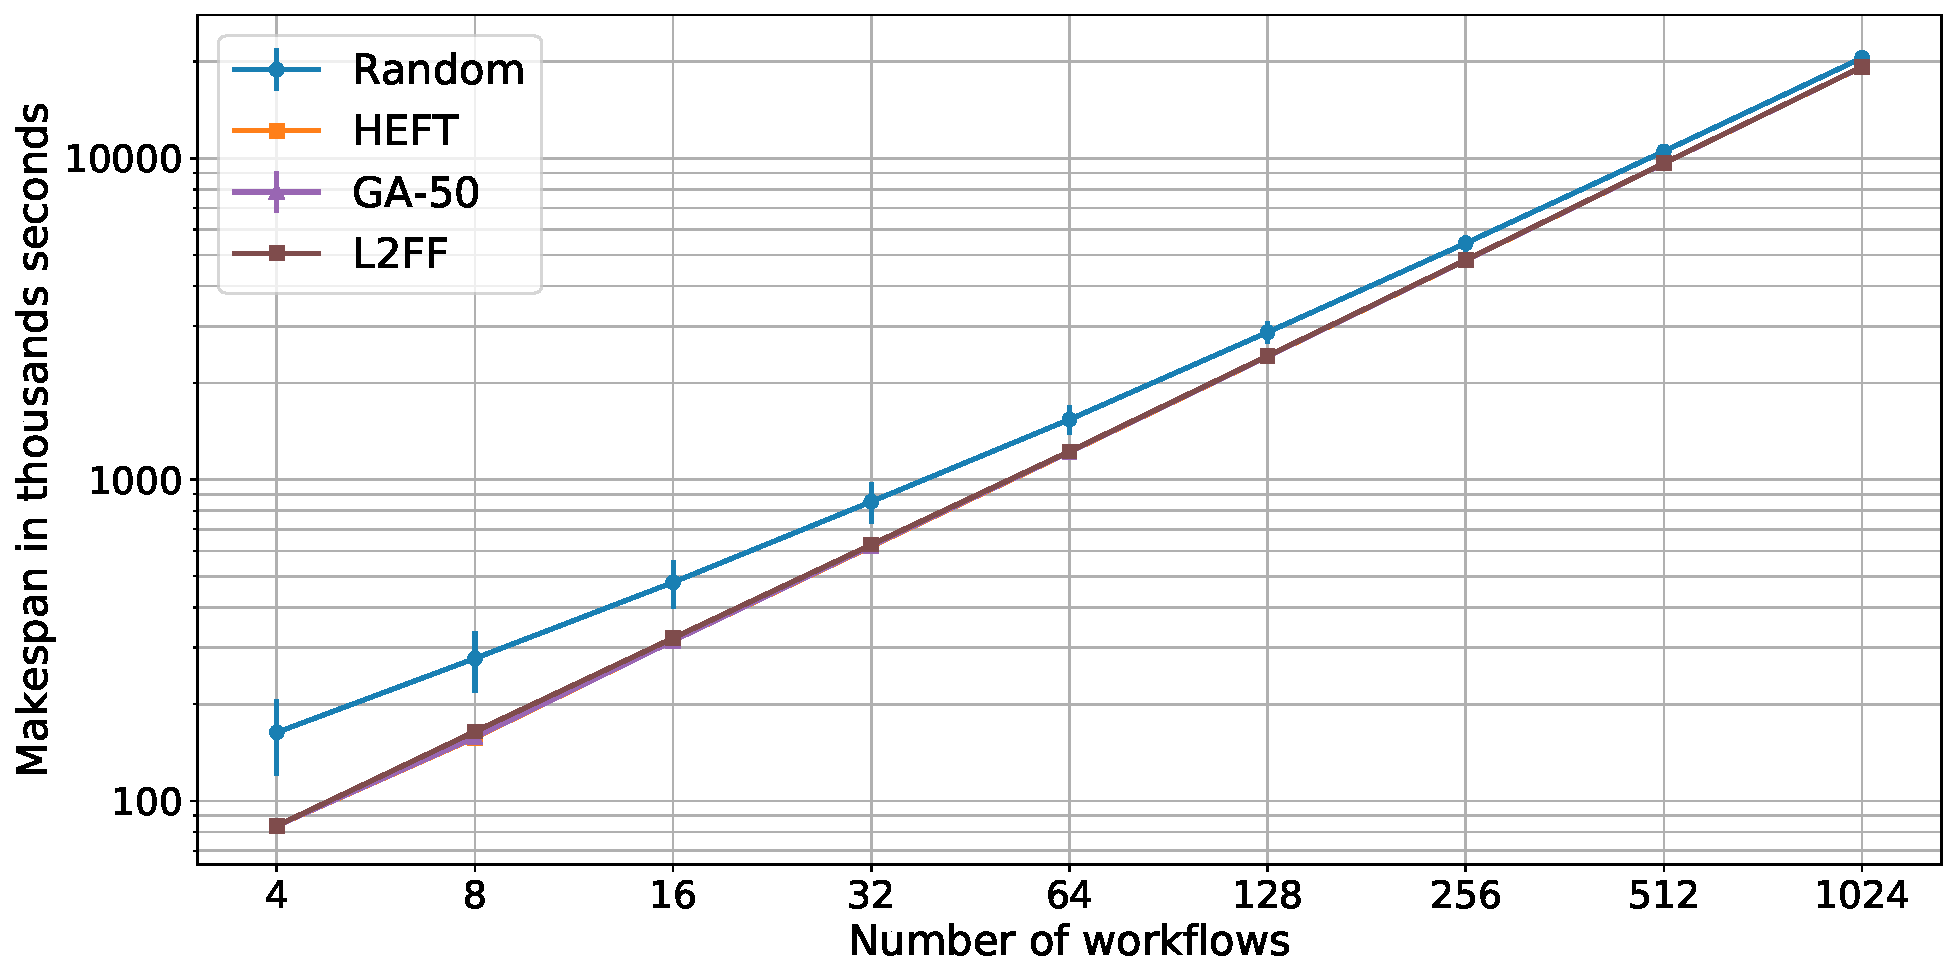
\includegraphics[width=.95\textwidth]{figures/campaign/StHeteroCampaigns_4StHomoResources.pdf}
        \caption{}
        \label{fig:StHeteroCampaigns_4StHomoResources}
    \end{subfigure}\\
    ~ 
    \begin{subfigure}[b]{0.85\textwidth}
        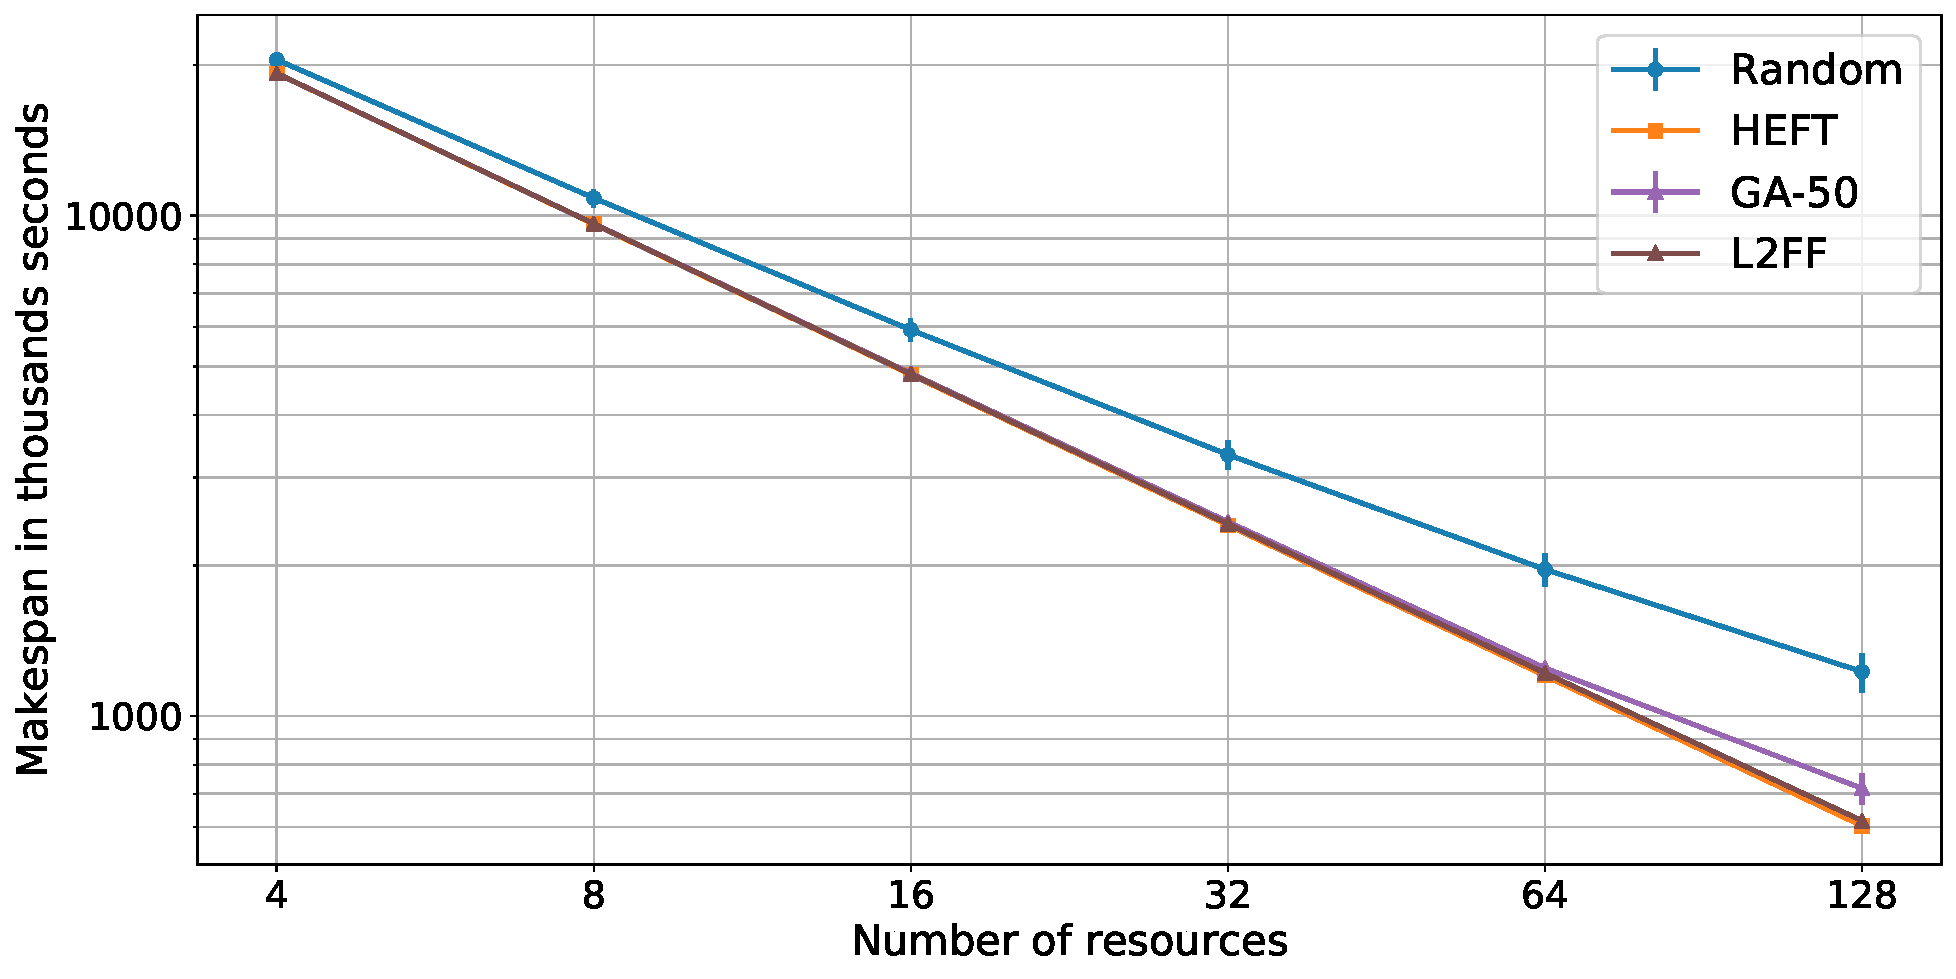
\includegraphics[width=.95\textwidth]{figures/campaign/HomogeResources_StHeteroCampaigns.pdf}
        \caption{}
        \label{fig:StHomoResources_StHeteroCampaigns}
    \end{subfigure}
    \caption{~\ref{fig:StHeteroCampaigns_4StHeteroResources}) Makespan of increasing number of heterogeneous worklfows on static homogeneous resources;
        ~\ref{fig:StHeteroResources_StHeteroCampaigns}) Makespan of heterogeneous campaign on different number of static homogeneous resources.}
    \label{fig:het_het_analysis}
\end{figure*}

Figure~\ref{fig:het_het_analysis} shows the performance of the three algorithms for a campaign with heterogeneous workflows on homogeneous resources.
Workflows are heterogeneous in terms of size, i.e., number of operations or total execution time.
We draw heterogeneous workflows from a normal distribution with a mean of 75000 and sigma 4900 execution time when executed on a resource with 1Peta-Flop performance.
Campaigns from the polar sciences are utilizing  data sets of imagery that are captured using the sensors over the same region.
It is expected then that the total size of these datasets will not change significantly and as a consequence the execution time of the workflows will not be considerably different.

The performance of the algorithms is not significantly different from the case of homogeneous workflows.
HEFT provides marginally better makespan from L2FF and the genetic algorithm.
This is because of the deterministic behavior of HEFT as well as the knowledge it creates for when resources are available.
L2FF has no notion of when a resource is available and the genetic algorithm creates some uncertainty due to the initial random placement of workflows on resources.


\begin{figure*}[ht!]
    \centering
    \begin{subfigure}[b]{0.85\textwidth}
        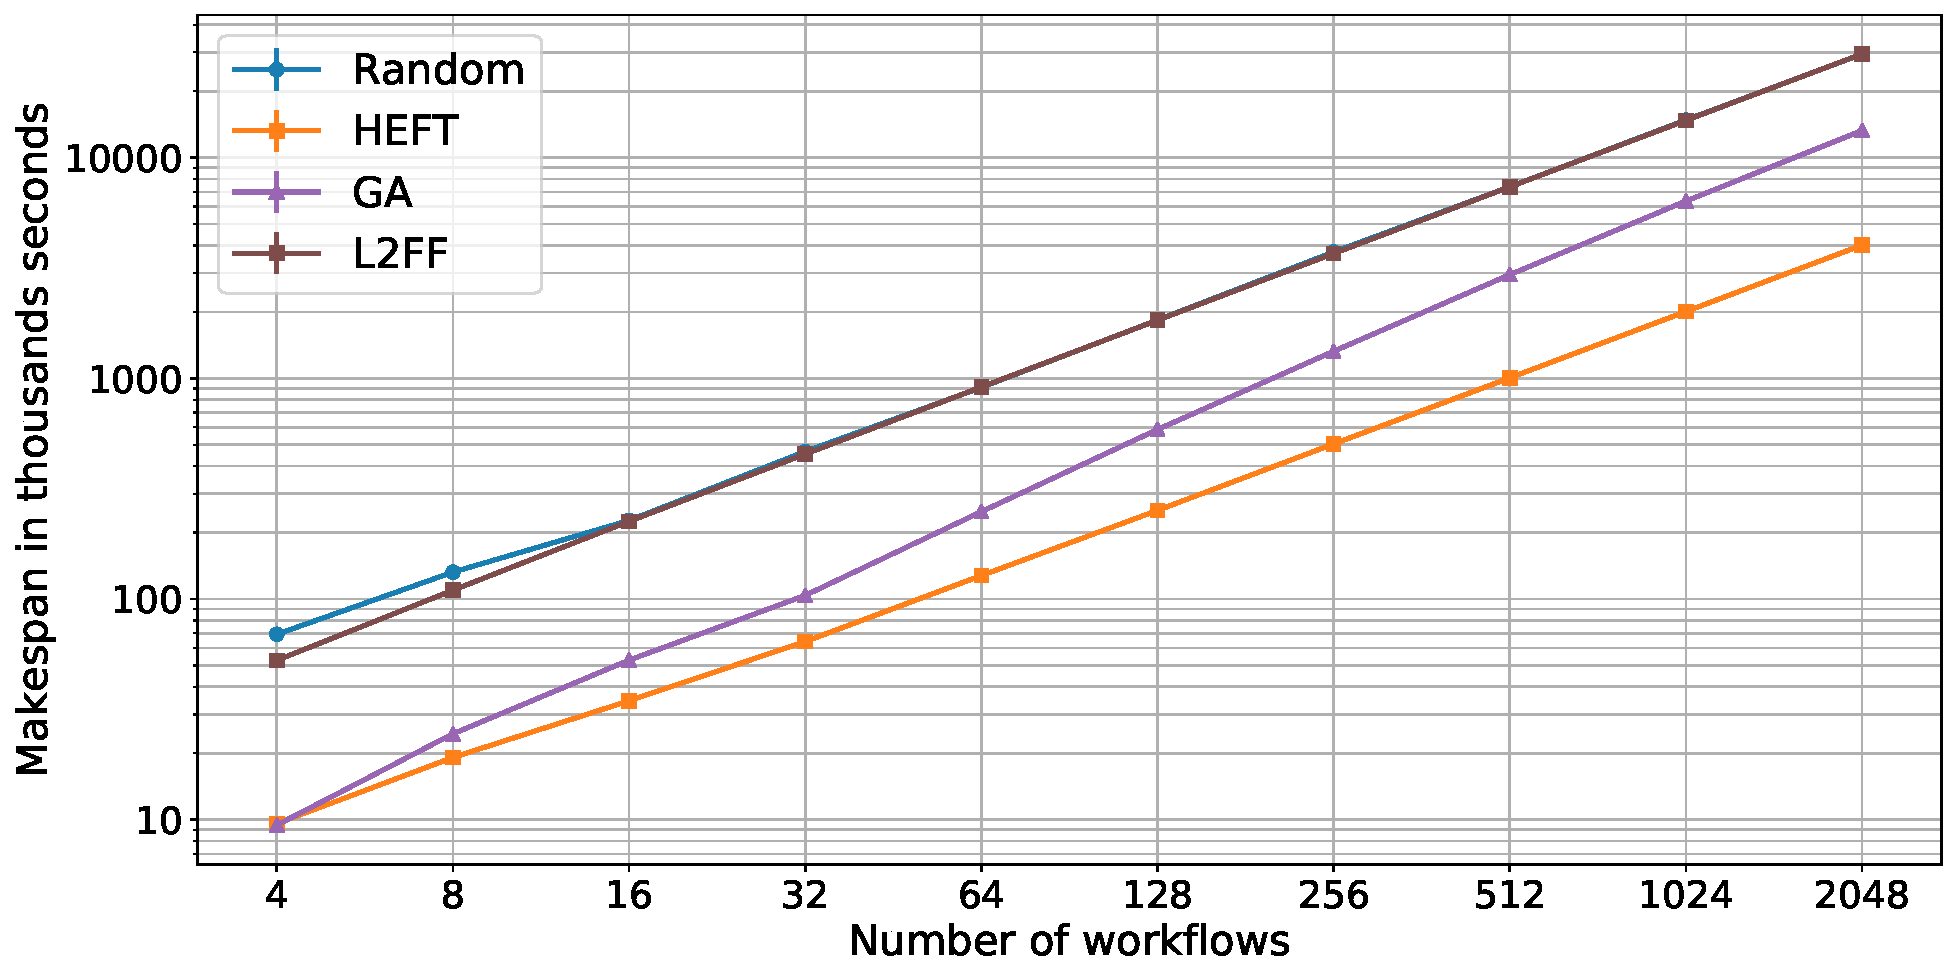
\includegraphics[width=.95\textwidth]{figures/campaign/StHeteroCampaigns_4StHeteroResources.pdf}
        \caption{}
        \label{fig:StHeteroCampaigns_4StHeteroResources}
    \end{subfigure}\\
    ~ 
    \begin{subfigure}[b]{0.85\textwidth}
        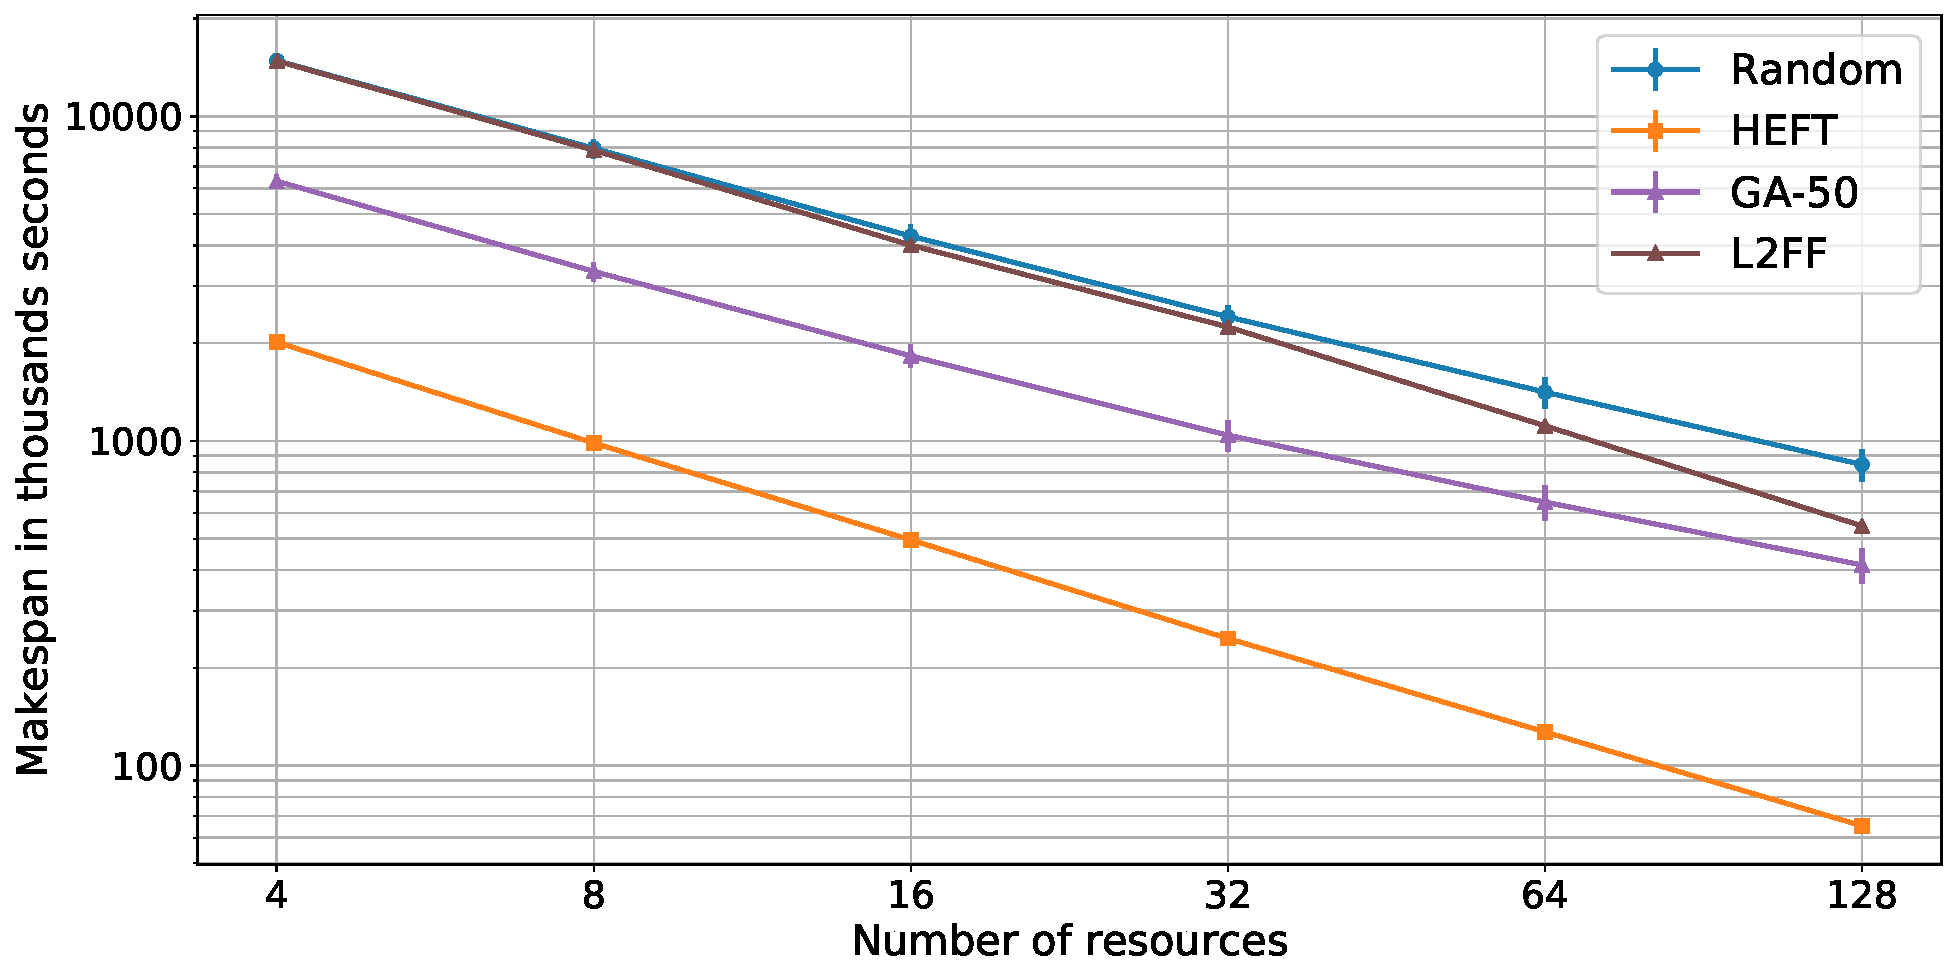
\includegraphics[width=.95\textwidth]{figures/campaign/StHeteroResources_StHeteroCampaigns.pdf}
        \caption{}
        \label{fig:StHeteroResources_StHeteroCampaigns}
    \end{subfigure}
    \caption{~\ref{fig:StHeteroCampaigns_4StHeteroResources}) Makespan of increasing number of heterogeneous worklfows on static heterogeneous resources;
        ~\ref{fig:StHeteroResources_StHeteroCampaigns}) Makespan of heterogeneous campaign on different number of static heterogeneous resources..}
    \label{fig:heter_analysis}
\end{figure*}

Figure~\ref{fig:heter_analysis} show the performance of the algorithms when heterogeneous resources are introduced.
Resources are being drawn from the distributions shown in Fig.~\ref{fig:heter_res}.
Specifically, for every 4 resources there is a Bridges, a Comet, a Stampede 2 and a Frontera like resource resulting to $k / 4$ single type resource with $k$ the total number of resources.

HEFT due to its knowledge of  resource availability and its deterministic behavior of calculating the makespan has the best performance of the three algorithms.
GA and L2FF are more sensitive to resource heterogeneity than HEFT.
The GA randomness in the initialization shows that the algorithm is not able to evolve to a makespan close to HEFT at least in 1oo iterations.
This also contributed in even worse performance from GA when the number of resources increases.
L2FF is more sensitive to resource heterogeneity compared to GA up to 128 resources. 
Although, we expect that L2FF will eventually produce better makespan than the genetic algorithm.
L2FF assigns $N \mod k$ workflows per resource, where $N$ the number of workflows in a campaign and $k$ the number of resources, while GA may produce a plan that may under-utilize or not use a resource completely.
This can be seen in figure~\ref{fig:res_util} where GA-50 did not utilize a Comet-like resource at all (Resource ID 37).

\begin{figure}[ht!]
    \centering
    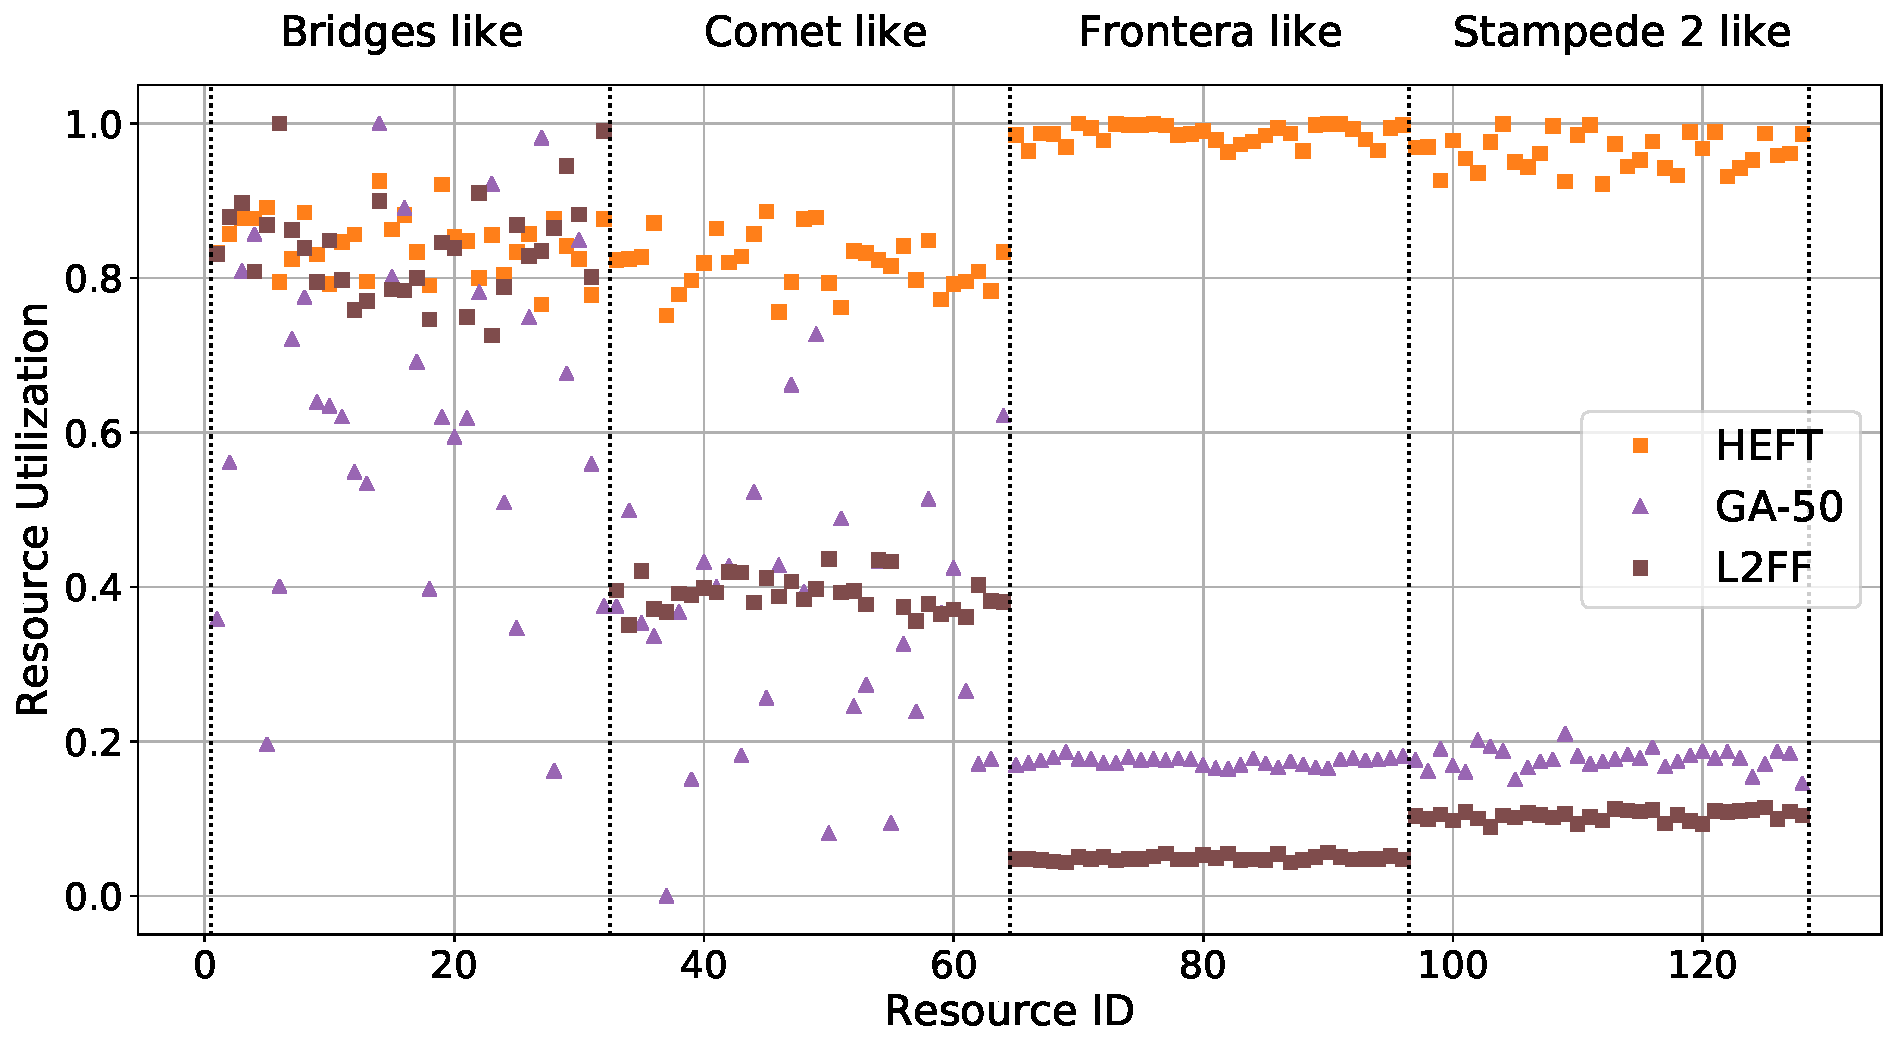
\includegraphics[width=.95\textwidth]{figures/campaign/HeteroResources_StHeteroCampaigns_Utils.pdf}
    \caption{Resource utilization for the best makespan from HEFT, GA-50 and L2FF for 1204 workflows and 128 heterogeneous resources.}
    \label{fig:res_util}
\end{figure}

Figure~\ref{fig:res_util} shows that HEFT is able to utilize as much as possible all the resources with almost full utilization of the fastest resources.
L2FF also utilizes all the resources, but under utilizes the faster ones due to it lack of knowledge for resource availability.
GA evolves to a plan that tries to utilize as much as possible the faster resources.
Having said that it can over utilize slower resources if more workflows are randomly assigned to those.

In general, algorithms that prioritize workflows based on their size and make deterministic decisions would provide the better makespan when a campaign is executed on homogeneous resources.
When resources are heterogeneous and distinct, algorithms that know when a resource is available provide better makespan for small number of resources.
As the number of resources increase non-deterministic algorithms will eventually not perform as well.
This allows to conclude that deterministic planning algorithms that produce or have the most knowledge about a campaign and the available resources are the ones that should be used on static resources..


\subsection{Experiment 2: Measuring makespan sensitivity on dynamic resources}

High performance computing resource performance is affected by a number of factors.
The shared filesystem and network performance, for example, changes based on I/O patterns and network congestion~\cite{brown2018interference}.
The performance of the CPUs and GPU of individual nodes are subject to policies that may allow multiple users on the same node, change CPU clock frequencies based on temperature and more.
As a result, the performance of a resource during the execution of a workflow can be different from the one a planning algorithm is expecting and thus dynamic.

The second experiments measures how sensitive is the plan produced by each algorithm to resource dynamicity.
We assume that the dynamic performance is drawn by a normal distribution where the mean performance is defined by the performance of the specific resource when it is considered static.
The variance is such that $3\sigma$ from the mean almost 20\% away from the mean.
Figure~\ref{fig:dynamic_res} shows an example of the distribution for mean equals to 1 and sigma equals to 0.06.

\begin{figure}[ht!]
    \centering
    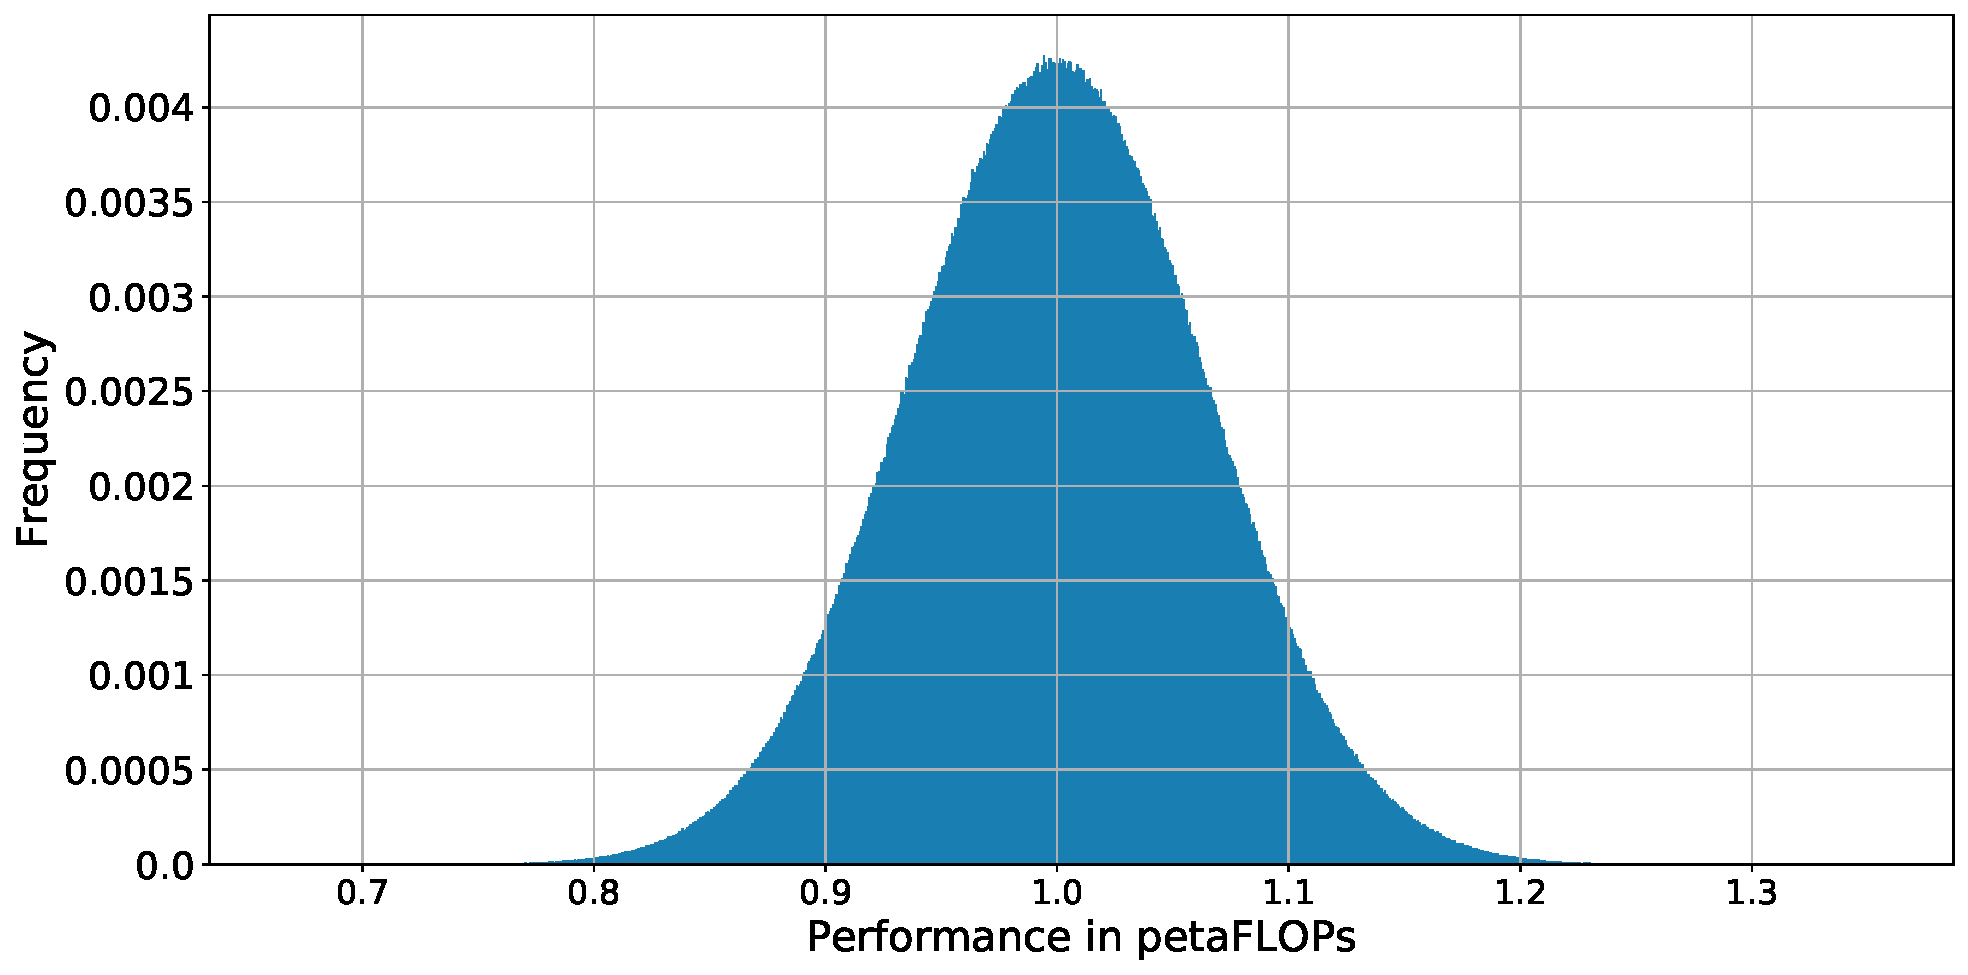
\includegraphics[width=.95\textwidth]{figures/campaign/DynRes.pdf}
    \caption{Resource performance distribution of a dynamic resource with 1 Peta-Flops average performance.}
    \label{fig:dynamic_res}
\end{figure}

We executed with the same configurations as in Experiment~1. 
Figure~\ref{fig:dyn_hetero_analysis} shows the performance of each algorithm when workflows are heterogeneous and resources are heterogeneous and dynamic.
Comparing with Figure~\ref{fig:het_het_analysis} we understand that all makespans are affected by resource dynamicity.
One important note is that HEFT due to its deterministic behavior and knowledge about resource availability still offers the better makespan compared to the other two algorithms.
A random plan provides still the worst makespan.

\begin{figure}[ht!]
    \centering
    \begin{subfigure}[b]{0.85\textwidth}
        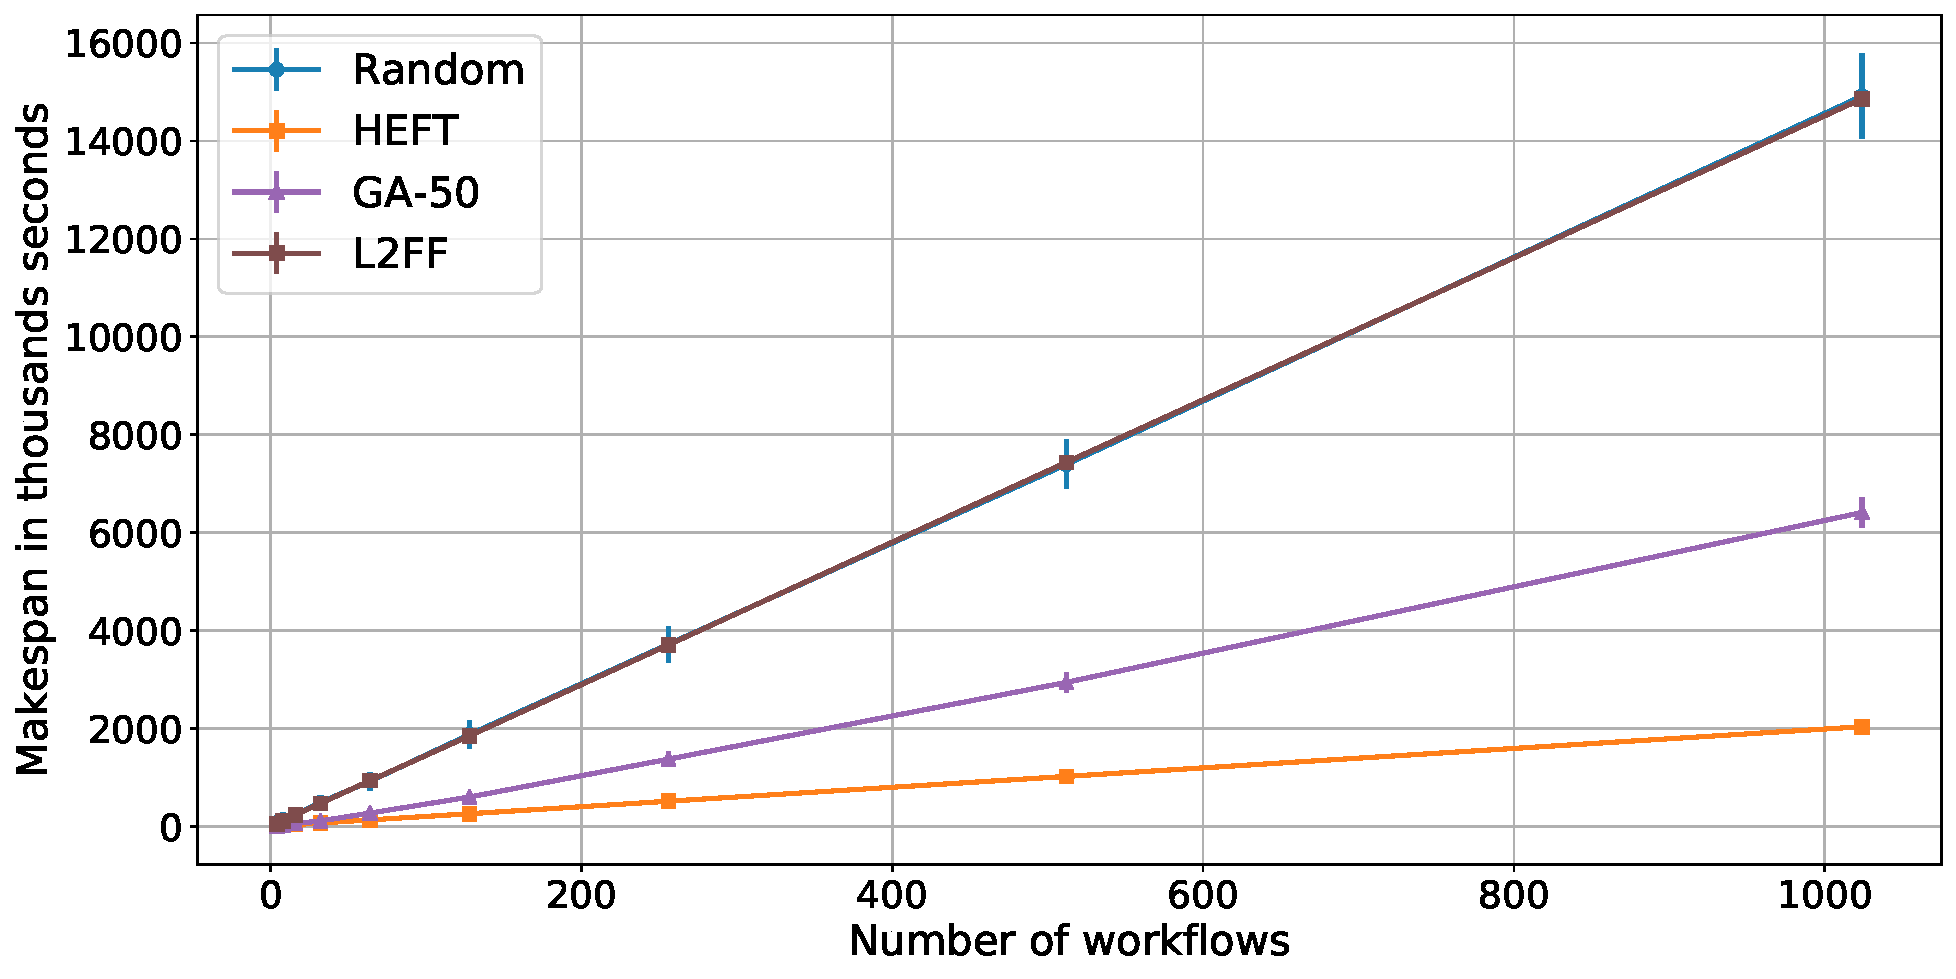
\includegraphics[width=.95\textwidth]{figures/campaign/StHeteroCampaigns_4DynHeteroResources.pdf}
        \caption{}
        \label{fig:StHeteroCampaigns_4DyHeteroResources}
    \end{subfigure}\\
    ~ 
    \begin{subfigure}[b]{0.85\textwidth}
        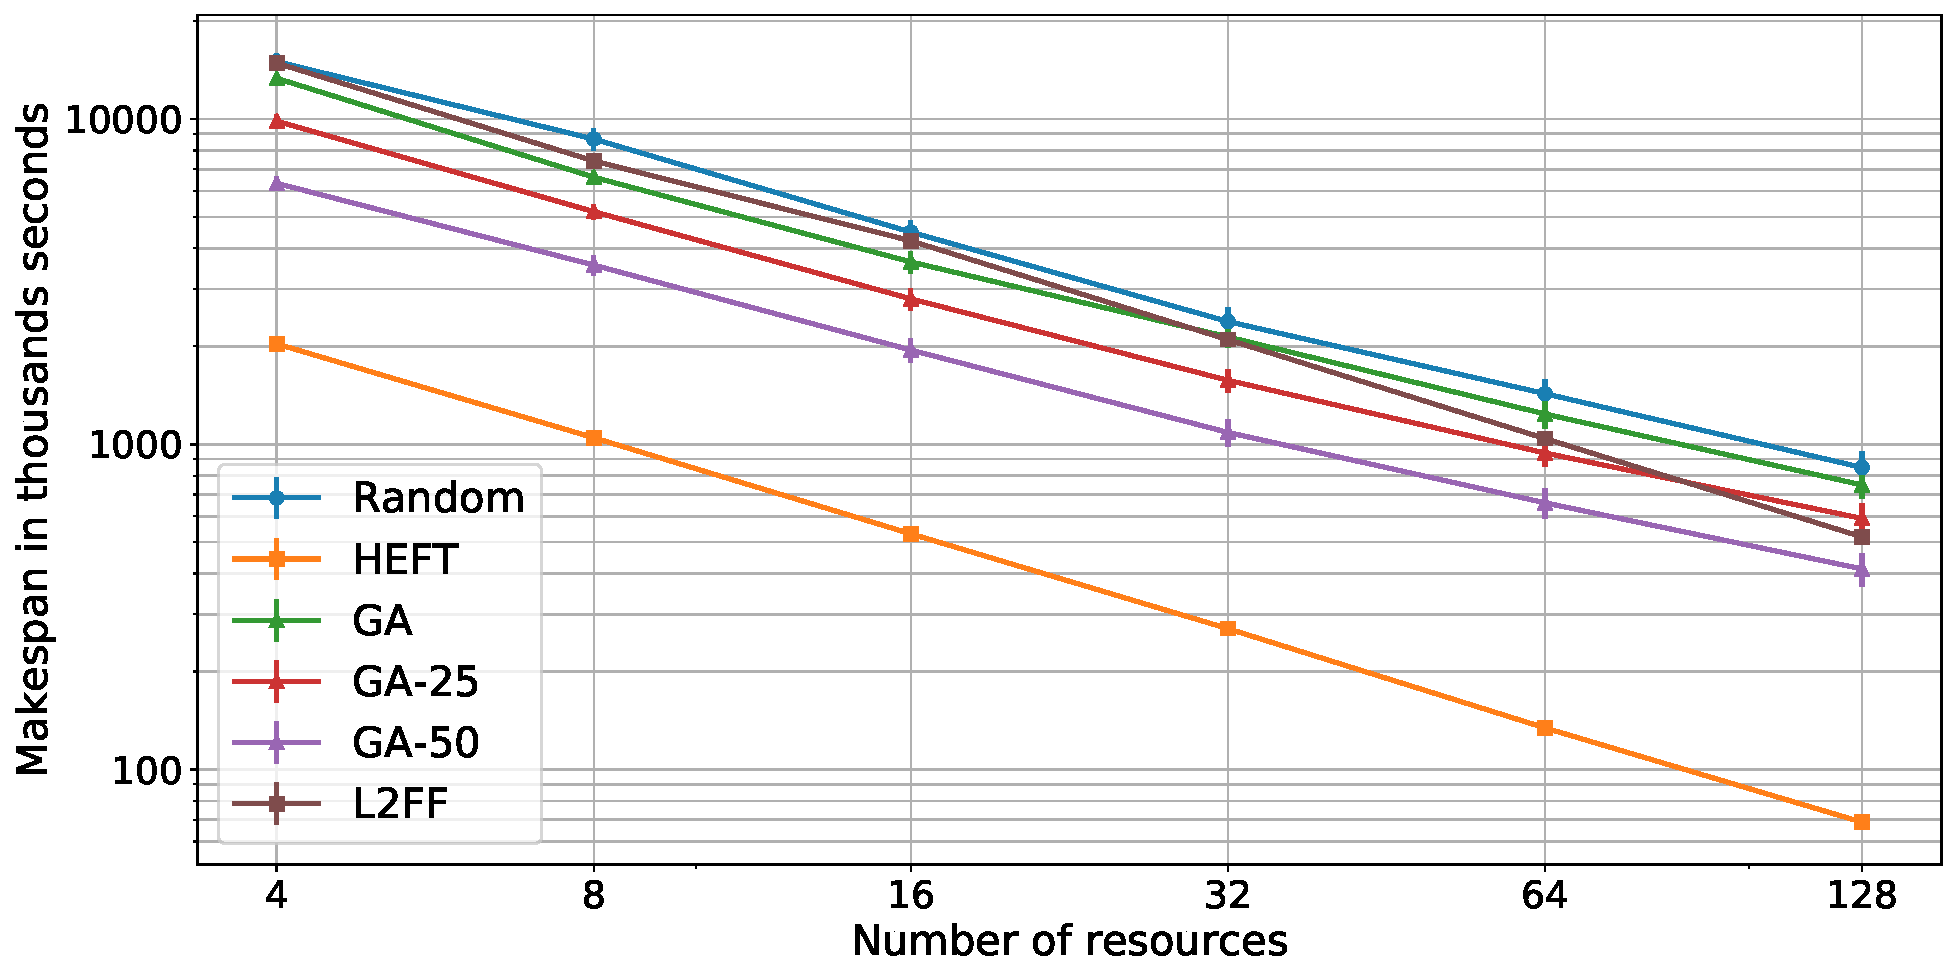
\includegraphics[width=0.95\textwidth]{figures/campaign/DynHeteroResources_StHeteroCampaigns.pdf}
        \caption{}
        \label{fig:DyHeteroResources_StHeteroCampaigns}
    \end{subfigure}
    \caption{~\ref{fig:StHeteroCampaigns_4DyHeteroResources} Makespan of increasing number of homogeneous workflows on homogeneous resources;
        ~\ref{fig:DyHeteroResources_StHeteroCampaigns} Makespan of homogeneous campaign on different number of homogeneous resources.}
    \label{fig:dyn_hetero_analysis}
\end{figure}

Figures~\ref{fig:dyn_homog_sens_analysis}, ~\ref{fig:dyn_hetero_homog_sens_analysis} and~\ref{fig:dyn_hetero_sens_analysis} show the results of our experiments for homogeneous workflows/ homogeneous resources, heterogeneous workflows/homogeneous resources and heterogeneous workflows/ heterogeneous resources.
In all configurations, we varied the number of workflows and the number of resources in the same way as experiment 1.

Figures~\ref{fig:StHomoCampaigns_4DyHomoResourcesSens} and~\ref{fig:DyHomoResources_StHomoCampaignsSens} show how sensitive are the algorithms when workflows and resources are homogeneous.
The random plan shows the least sensitivity as for both cases, varying the varying the number of workflows (Fig.~\ref{fig:StHomoCampaigns_4DyHomoResourcesSens} and varying the number of resources (Fig.~\ref{fig:DyHomoResources_StHomoCampaignsSens}).
All three algorithms are affected the same way by the introduced dynamicity.
One important note is that the variability of the makespan is not more than 10\% in all cases.
The algorithmic sensitivity decreases as the number of workflows increase when the number of resources is constant.
In addition, it increases as the number of resources increase when the number of workflows remains constant.
This points us to the conclusion that the sensitivity of the algorithms is proportional to the ratio of workflows over resources.

\begin{figure}[ht!]
    \centering
    \begin{subfigure}[b]{0.85\textwidth}
        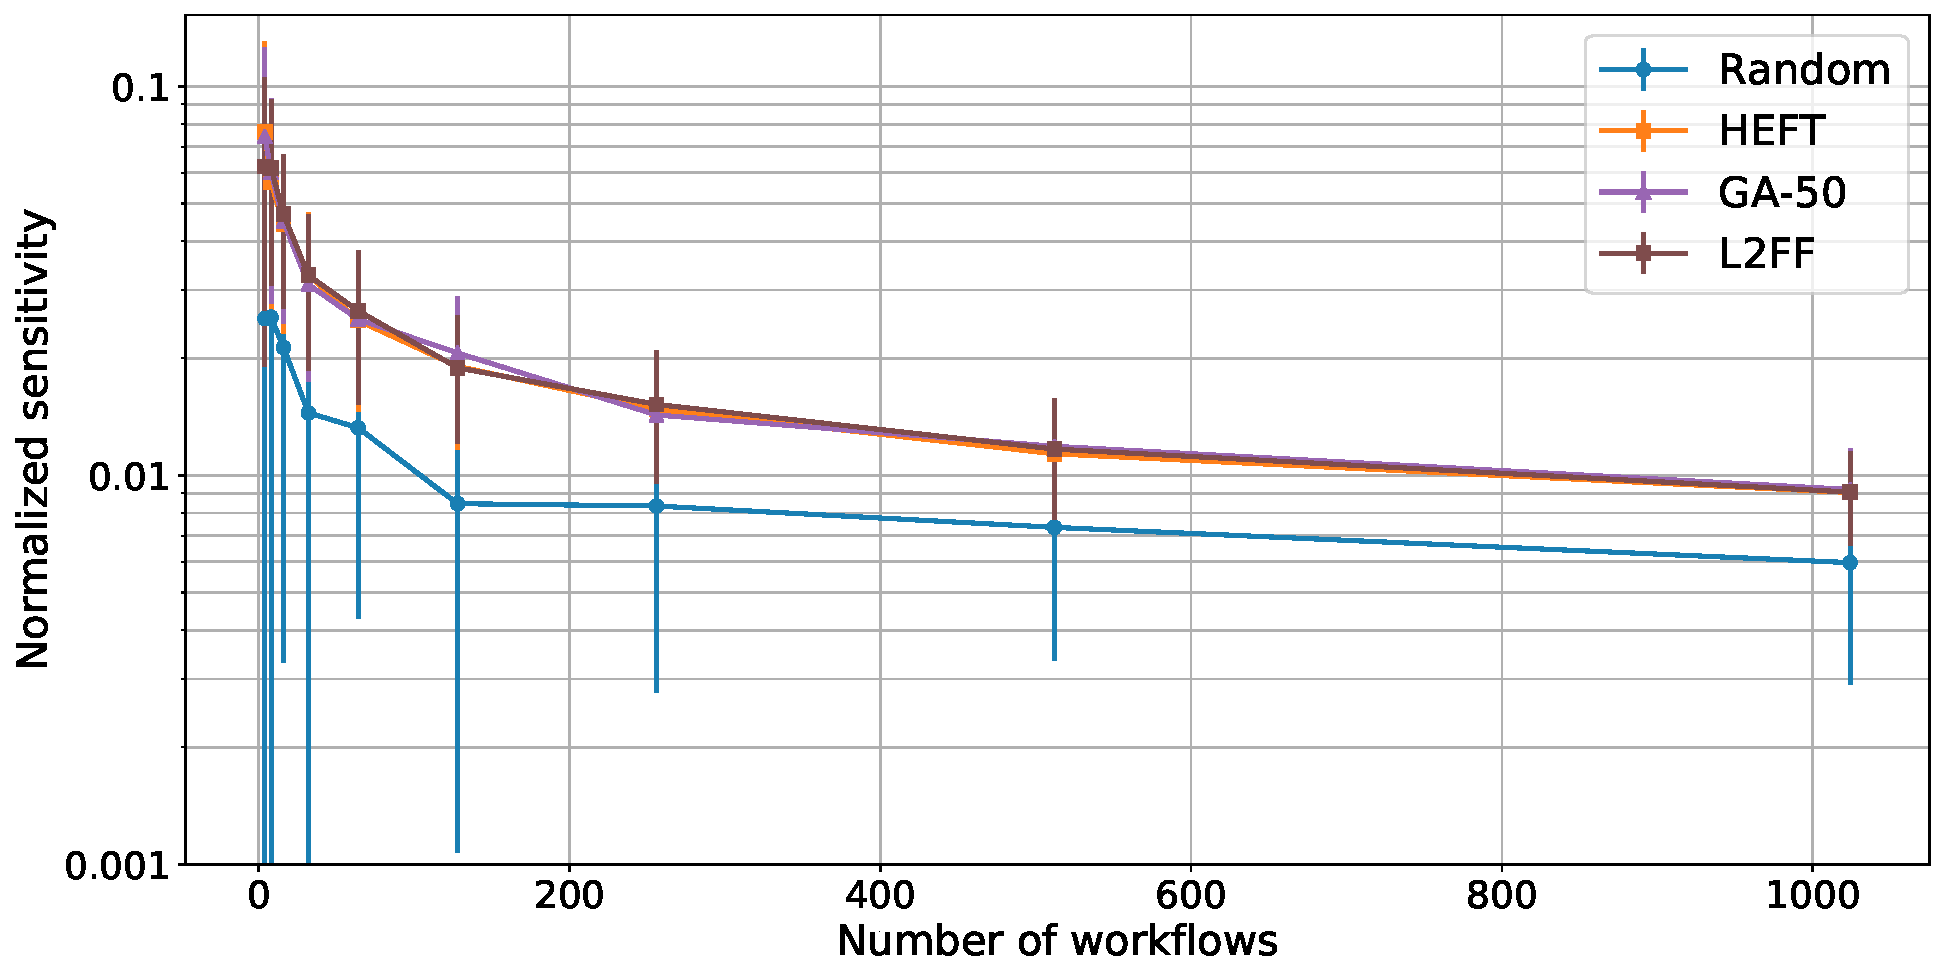
\includegraphics[width=.95\textwidth]{figures/campaign/StHomoCampaigns_4DynHomoResourcesSens.pdf}
        \caption{}
        \label{fig:StHomoCampaigns_4DyHomoResourcesSens}
    \end{subfigure}\\
    ~ 
    \begin{subfigure}[b]{0.85\textwidth}
        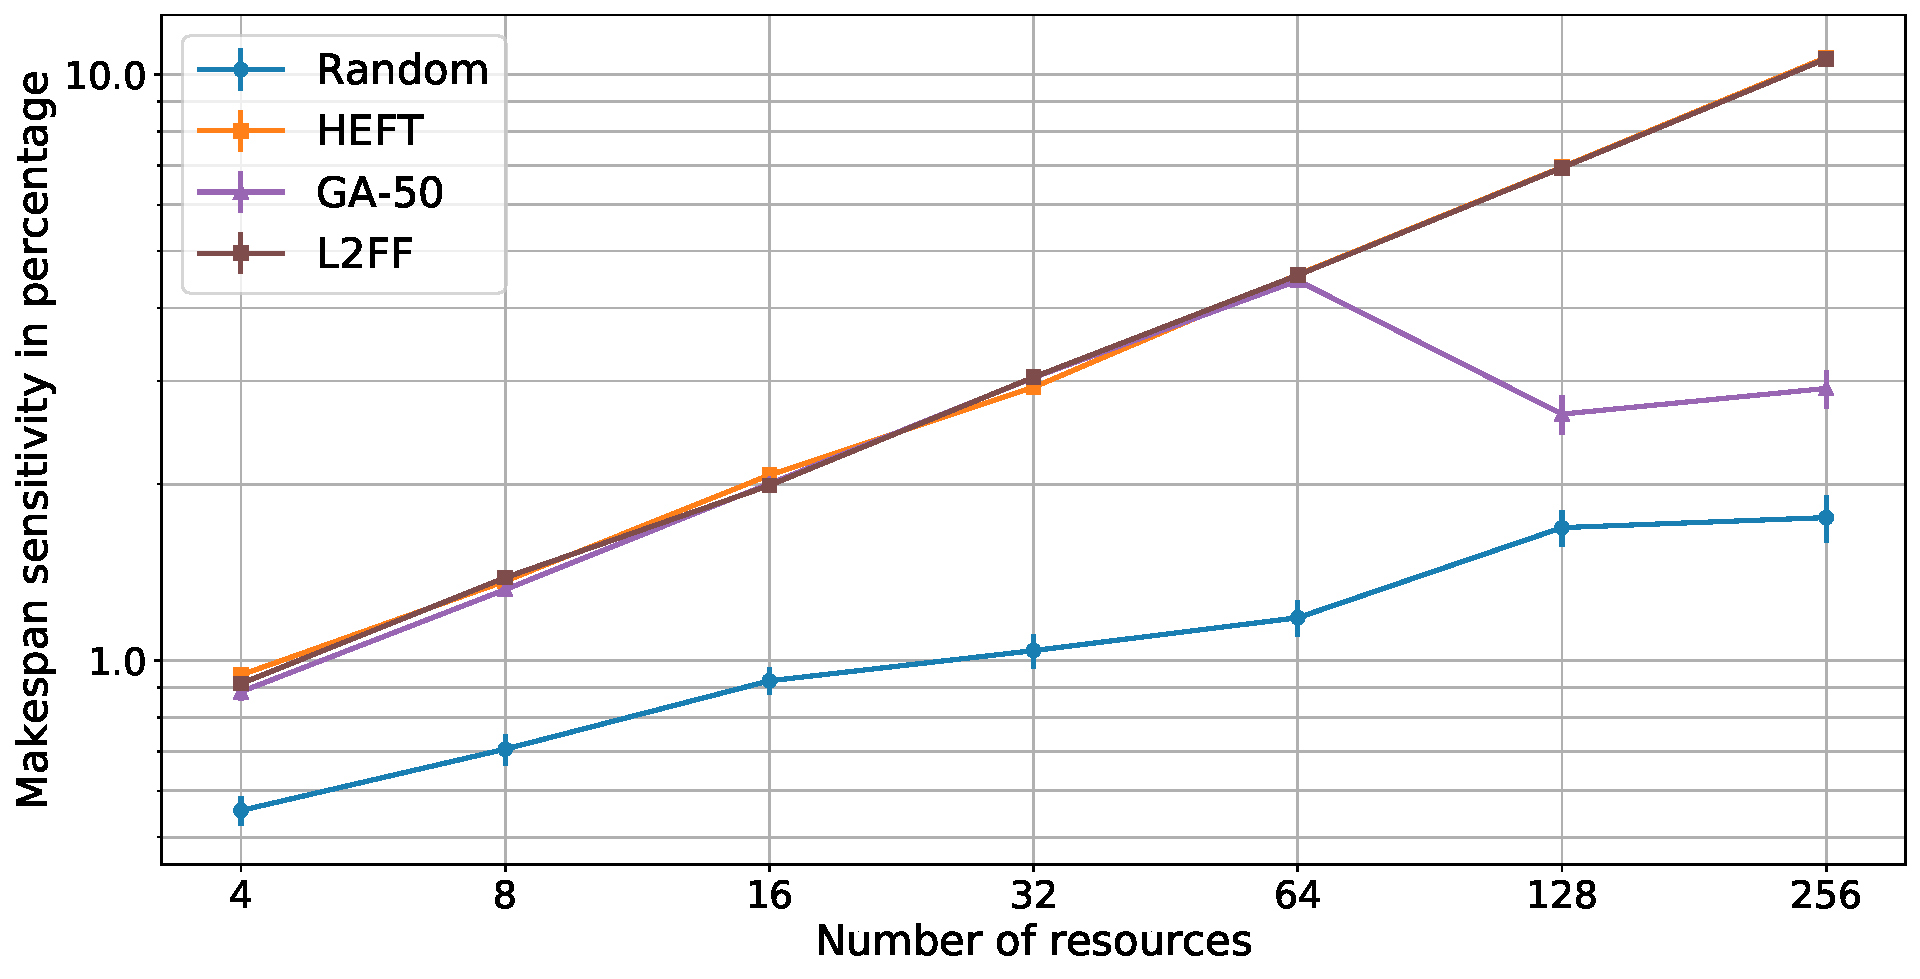
\includegraphics[width=0.95\textwidth]{figures/campaign/DynHomoResources_StHomoCampaignsSens.pdf}
        \caption{}
        \label{fig:DyHomoResources_StHomoCampaignsSens}
    \end{subfigure}
    \caption{~\ref{fig:StHomoCampaigns_4DyHomoResourcesSens} Normalized makespan sensitivity of increasing number of homogeneous workflows on homogeneous resources;
        ~\ref{fig:DyHomoResources_StHomoCampaignsSens} Normalized makespan sensitivity  of homogeneous campaign on different number of homogeneous resources.}
    \label{fig:dyn_homog_sens_analysis}
\end{figure}

In figure~\ref{fig:dyn_hetero_homog_sens_analysis} we introduce workflow heterogeneity.
The algorithms makespan performance behavior is similar to the one shown in Fig.~\ref{fig:het_het_analysis}.
Despite the fact, HEFT show the largest sensitivity when varying the number of workflows and when varying the number of resources.
The genetic algorithm shows similar sensitivity with HEFT when the number of workflows but tends to be less sensitive when the number of resources increase.
The genetic algorithm assigns a percentage of workflows to resources randomly which in turn makes it less sensitive to resource dynamicity, especially when the number of resources is large.

L2FF shows a similar behavior with HEFT, especially when the number of resources changes, despite being less sensitive.
In addition, the genetic algorithm sensitivity gets closer to that of random when the number of resources increases.
Both L2FF and HEFT are deterministic and they produce always the same plan for a given campaign and set of resources.
This in turn results to an increasing sensitivity as the ratio of number of campaign size to number of resources is small.
In contrast, the random initial placement of GA allows it to create a plan that is less sensitive to dynamicity with the cost of slightly makespan, 725K seconds versus 643K and 649K seconds from HEFT and L2FF respectively.

\begin{figure}[ht!]
    \centering
    \begin{subfigure}[b]{0.85\textwidth}
        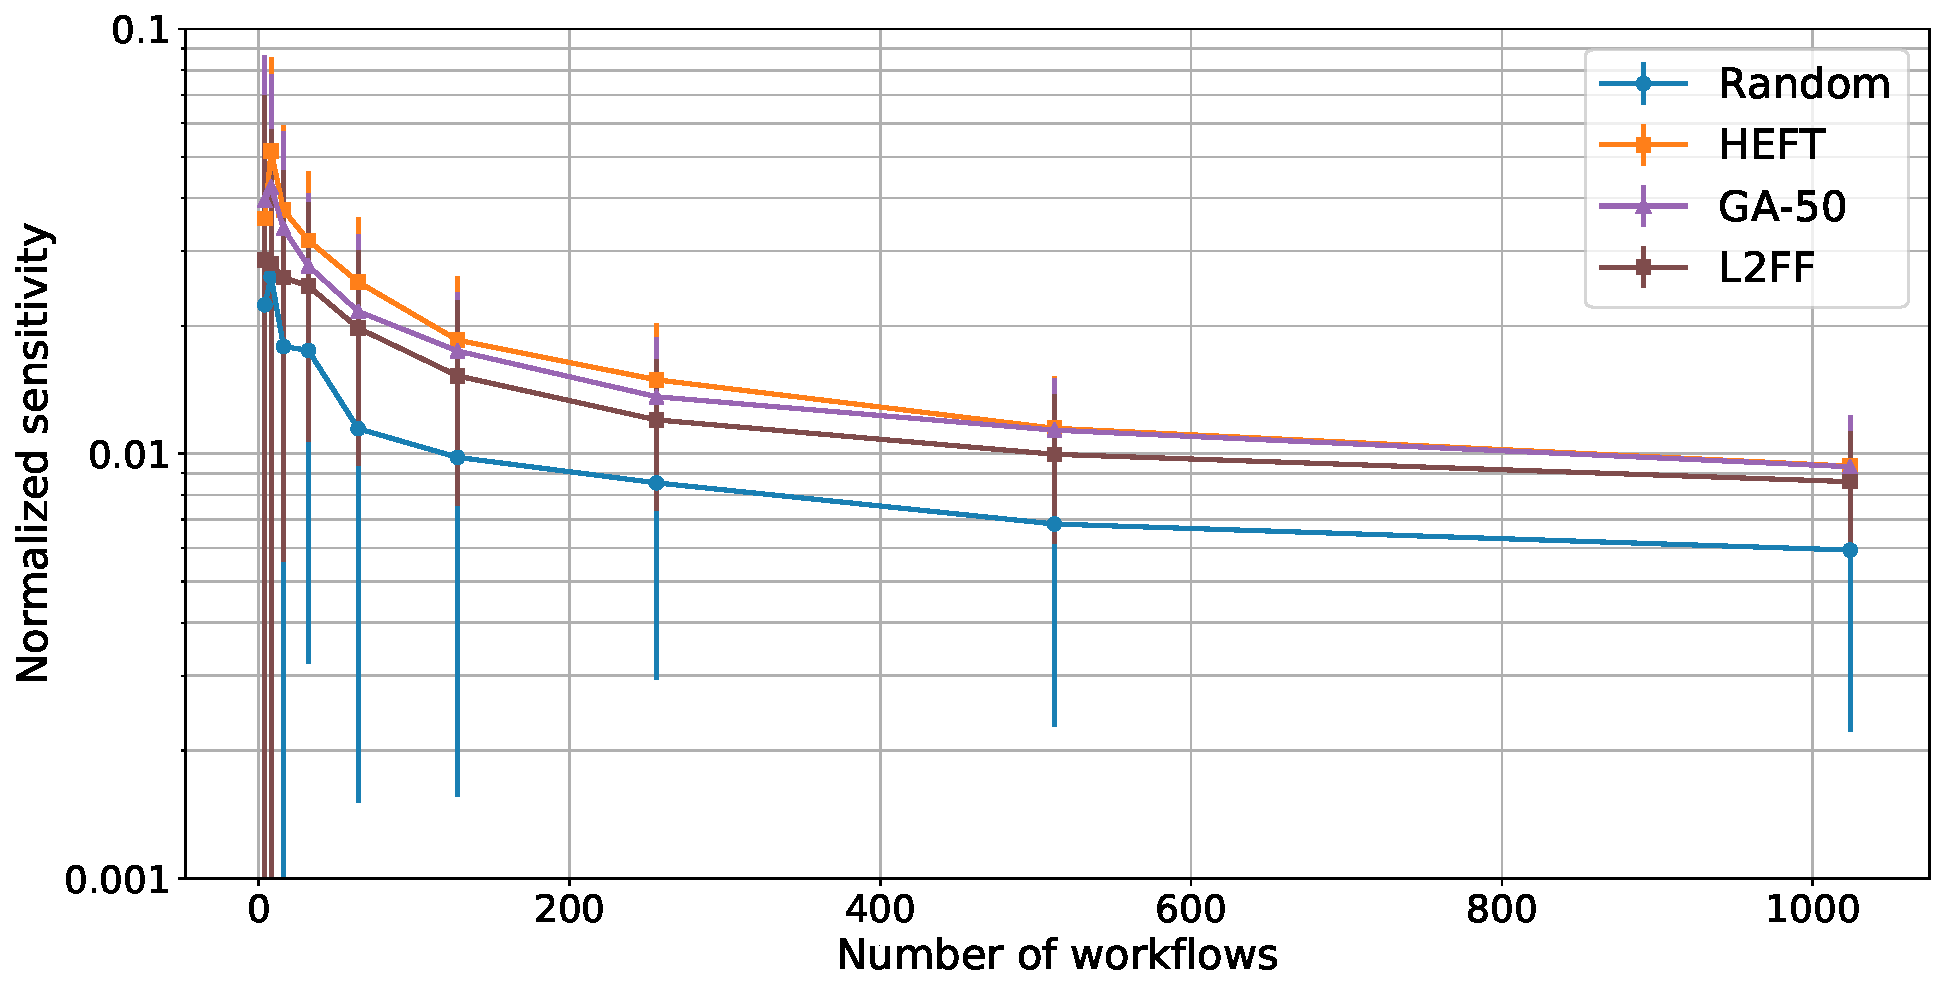
\includegraphics[width=.95\textwidth]{figures/campaign/StHeteroCampaigns_4DynHomoResourcesSens.pdf}
        \caption{}
        \label{fig:StHeteroCampaigns_4DynHomoResourcesSens}
    \end{subfigure}\\
    ~ 
    \begin{subfigure}[b]{0.85\textwidth}
        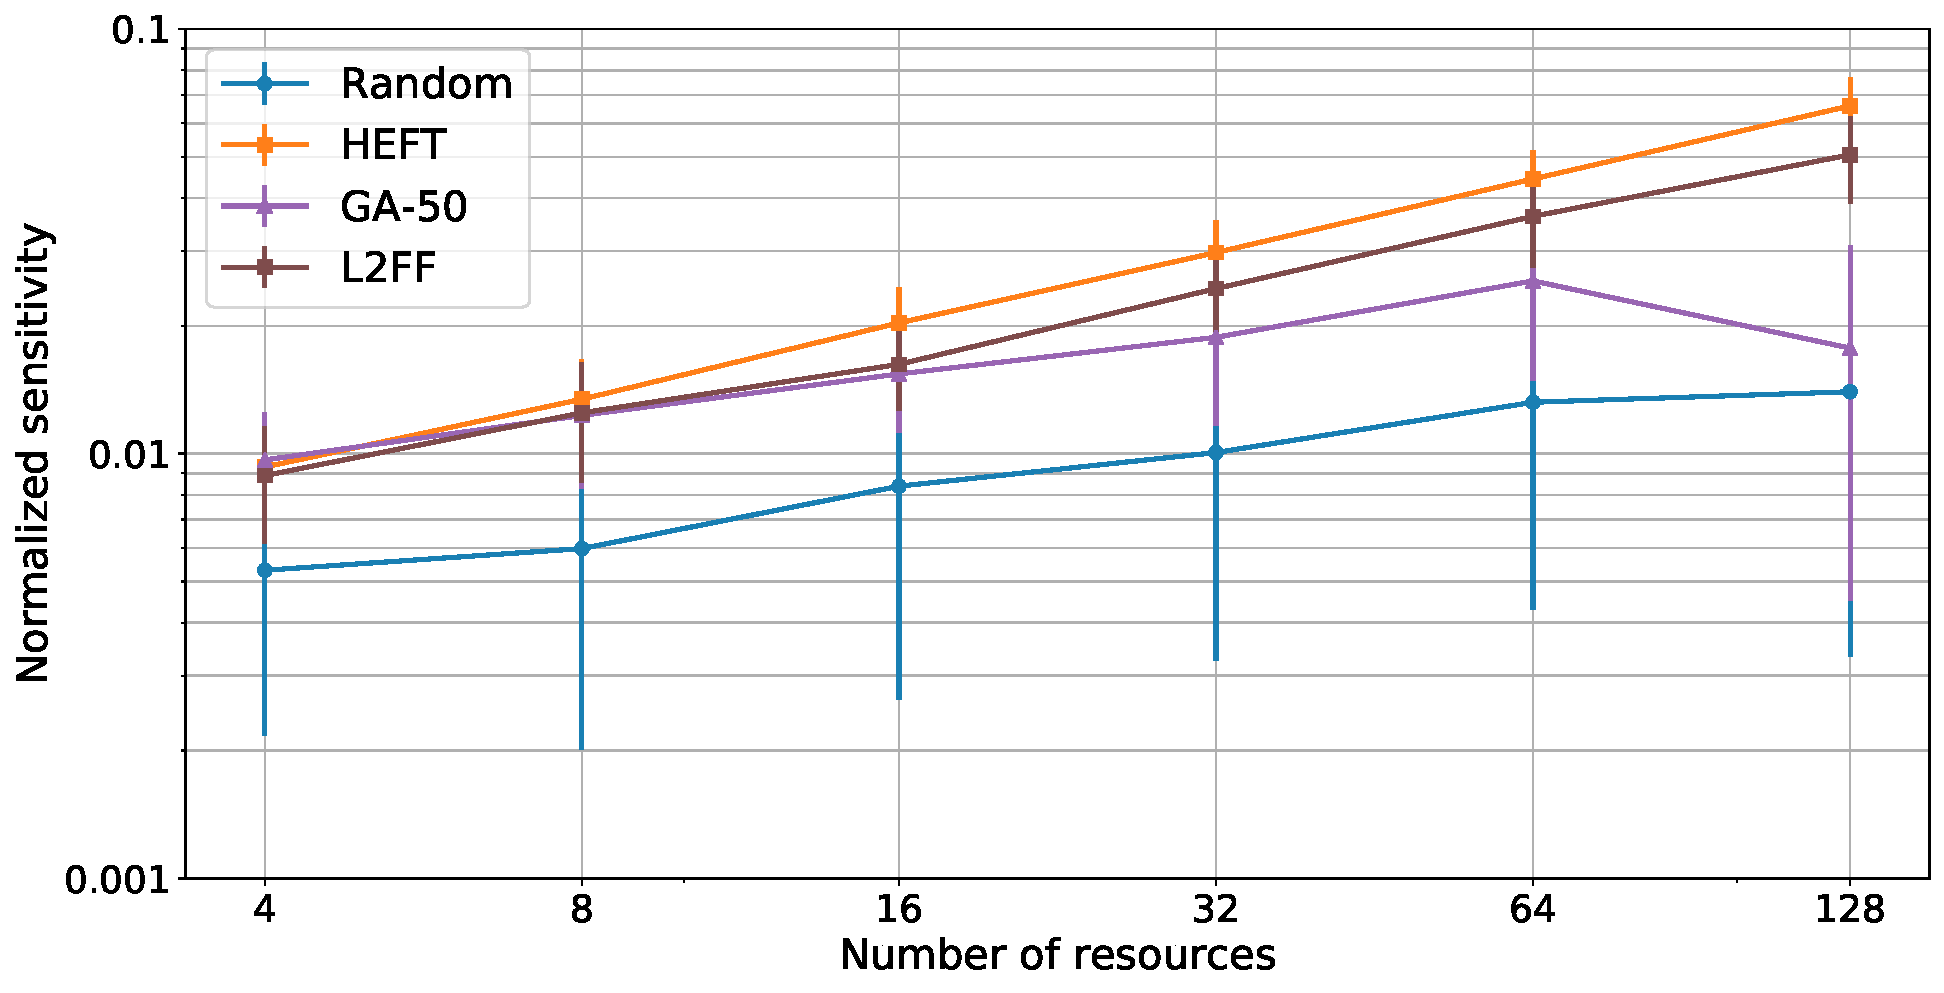
\includegraphics[width=0.95\textwidth]{figures/campaign/DynHomoResources_StHeteroCampaignsSens.pdf}
        \caption{}
        \label{fig:DynHomoResources_StHeteroCampaignsSens}
    \end{subfigure}
    \caption{~\ref{fig:StHeteroCampaigns_4DynHomoResourcesSens} Normalized makespan sensitivity  of increasing number of heterogeneous workflows on homogeneous resources;
        ~\ref{fig:DynHomoResources_StHeteroCampaignsSens} Normalized makespan sensitivity  of a heterogeneous campaign on different number of homogeneous resources.}
    \label{fig:dyn_hetero_homog_sens_analysis}
\end{figure}

Resource heterogeneity has a significant impact in the makespan as seen Experiment 1.
We expect resource dynamicity to reduce this impact.
As shown in Figure~\ref{fig:dyn_hetero_sens_analysis} this is not true.
The makespan is affected less than 10~\% despite the algorithm used.
HEFT shows the largest effect in the makespan.
GA and L2FF show similar impact with the random placement, however GA has produces a better plan than both (see Fig.~\ref{fig:dyn_hetero_analysis}), with significant difference when the ratio of campaign size to number of resources is large.

\begin{figure}[ht!]
    \centering
    \begin{subfigure}[b]{0.85\textwidth}
        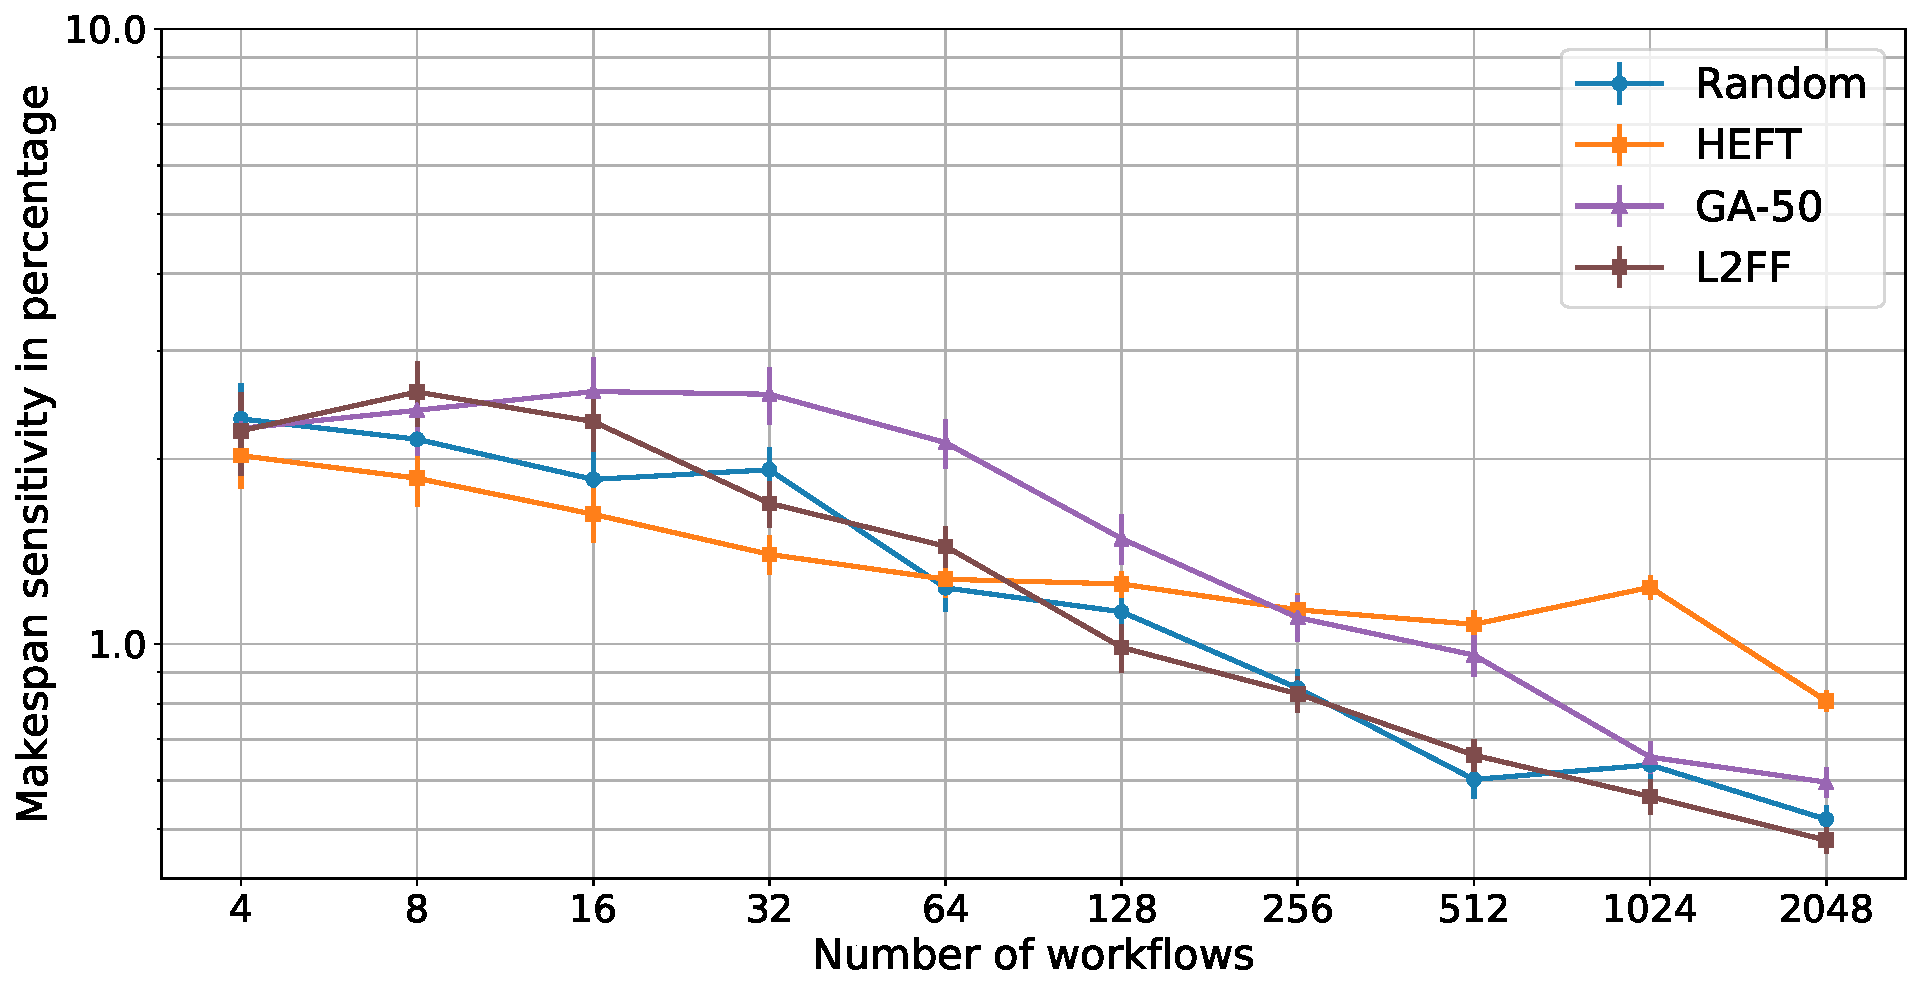
\includegraphics[width=.95\textwidth]{figures/campaign/StHeteroCampaigns_4DynHeteroResourcesSens.pdf}
        \caption{}
        \label{fig:StHeteroCampaigns_4DyHeteroResourcesSens}
    \end{subfigure}\\
    ~ 
    \begin{subfigure}[b]{0.85\textwidth}
        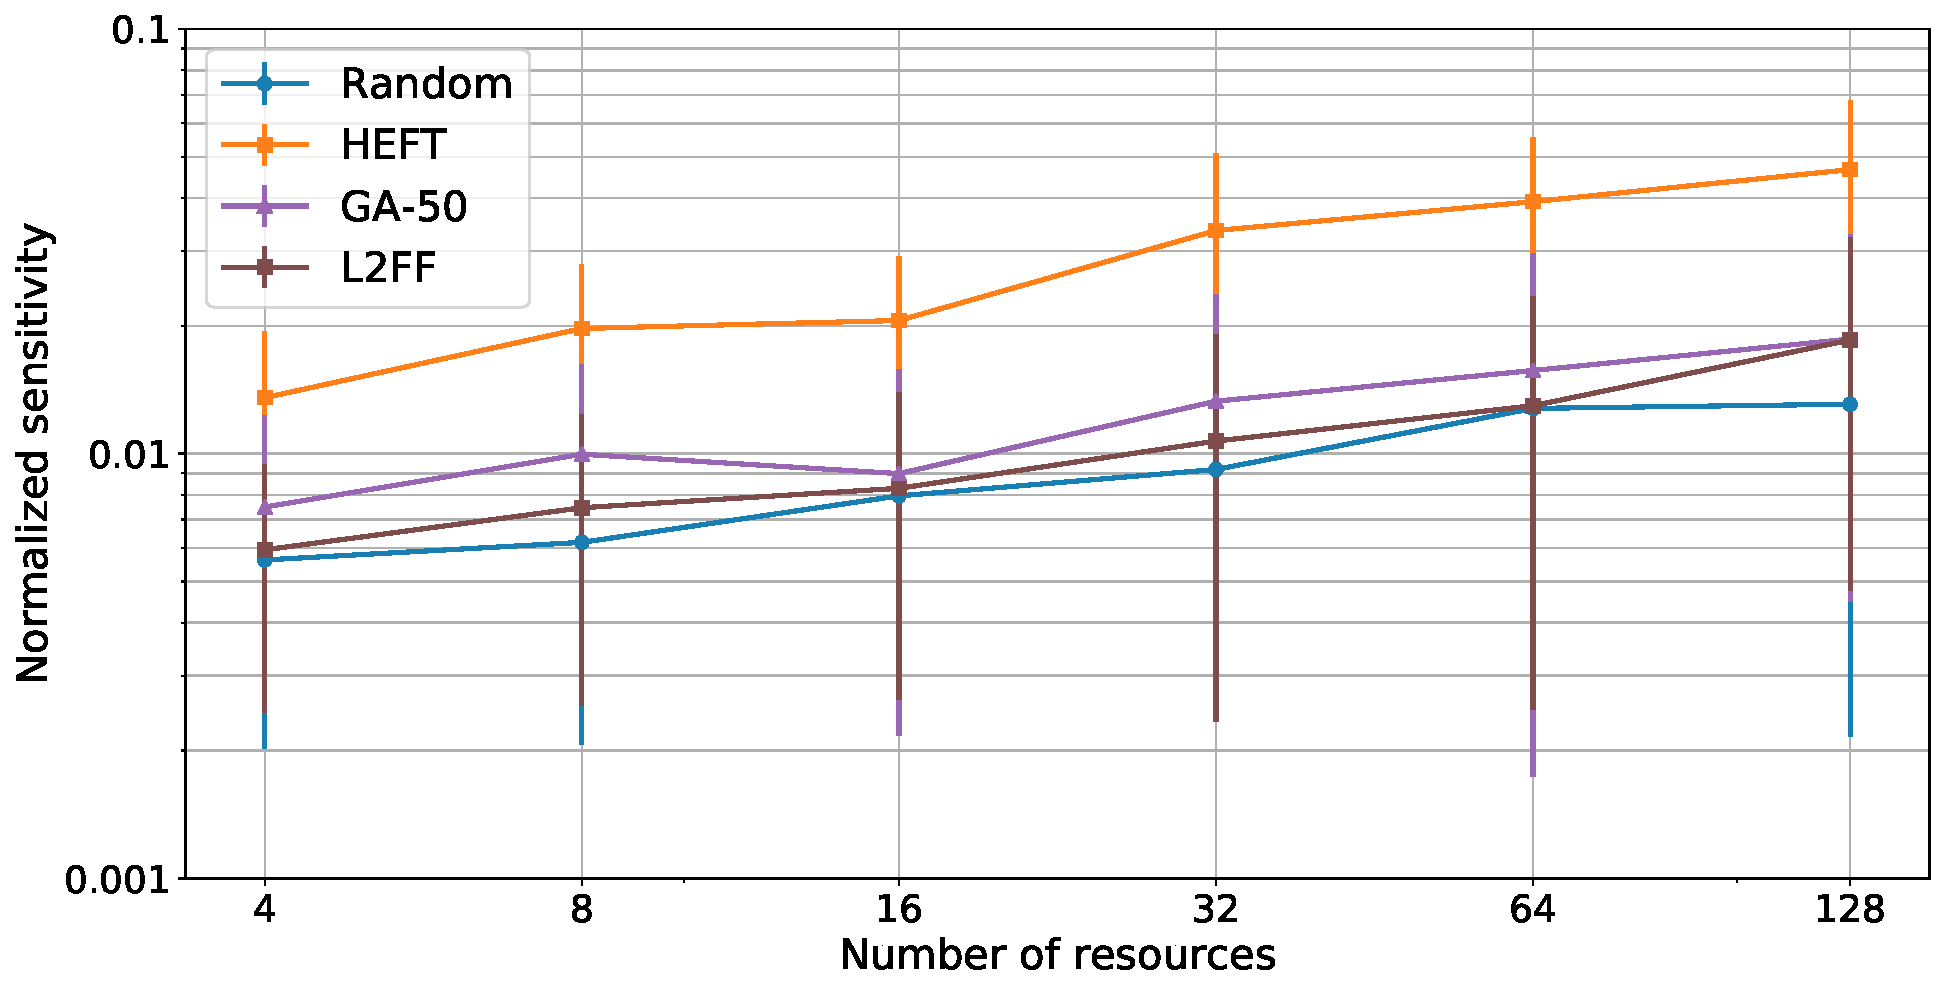
\includegraphics[width=0.95\textwidth]{figures/campaign/DynHeteroResources_StHeteroCampaignsSens.pdf}
        \caption{}
        \label{fig:DyHeteroResources_StHeteroCampaignsSens}
    \end{subfigure}
    \caption{~\ref{fig:StHeteroCampaigns_4DyHeteroResourcesSens} Normalized makespan sensitivity  of increasing number of heterogeneous workflows on heterogeneous resources;
    ~\ref{fig:DyHeteroResources_StHeteroCampaignsSens} Normalized makespan sensitivity  of heterogeneous campaign on different number of heterogeneous resources.}
    \label{fig:dyn_hetero_sens_analysis}
\end{figure}

This experiment measured the impact of resource dynamicity on the makespan produced by the selected algorithms.
Although resource dynamicity did not change the ranking of the algorithms, it shows that algorithms with strong assumptions about workflow number of operations, resource performance and resource availability are affected the most.
Furthermore, the impact of resource dynamicity is inverse proportional to the ratio of campaign size over number of resources.
Based on the assumptions an algorithm makes, resource heterogeneity can affect the impact dynamic resource may have on the makespan of the produced plan.
This experiment together with experiment 1 allow us to conclude that resource heterogeneity is the factors that affects the most the performance of the algorithms.


\subsection{Experiment 3: Measuring makespan sensitivity based workflow length uncertainty}

All of the selected algorithms, apart from the random, require information about number of operations or length of each workflow.
The user usually offers this kind of information either through a function or a single number drawn by empirical data.
When executing computational campaigns that process complex datasets, it is understandable that even the most accurate information can have some level of uncertainty.
This, in turn, means that execution plans may not produce the best possible makespan.
This experiment measures how sensitive are the plans produced by the selected algorithms for different levels of uncertainty.

We introduce workflow information uncertainty as the difference between the estimated and actual runtime of a workflow on a 1 Peta-flops resource.
Specifically, we denote as $u$ the level of uncertainty between $[0,1)$, $u'$ the uncertainty for a workflow drawn randomly from the range $[-u,u]$ and $w$ the estimated runtime of a workflow.
So the actual runtime of the workflow $w'$ is $ w' = w \times (1-u')$.

As shown in the previous experiments the algorithms show significant performance differences when heterogeneous resources are used.
As a result, we executed this experiment for heterogeneous workflows and heterogeneous static and dynamic resources for different levels of uncertainty.
We use normalized sensitivity as the selected metric for this experiment and measured it for uncertainty from 10~\% up to 90~\% with 10~\% step.
Figure~\ref{fig:inaccur_st} shows the results for static resources with figure~\ref{fig:InaccurStHeteroCampaigns_4StHeteroResourcesSens} varying the number of workflows and~\ref{fig:InaccurStHeteroResources_StHeteroCampaignsSens} varying the number of resources.

\begin{figure}[ht!]
    \centering
    \begin{subfigure}[b]{0.95\textwidth}
        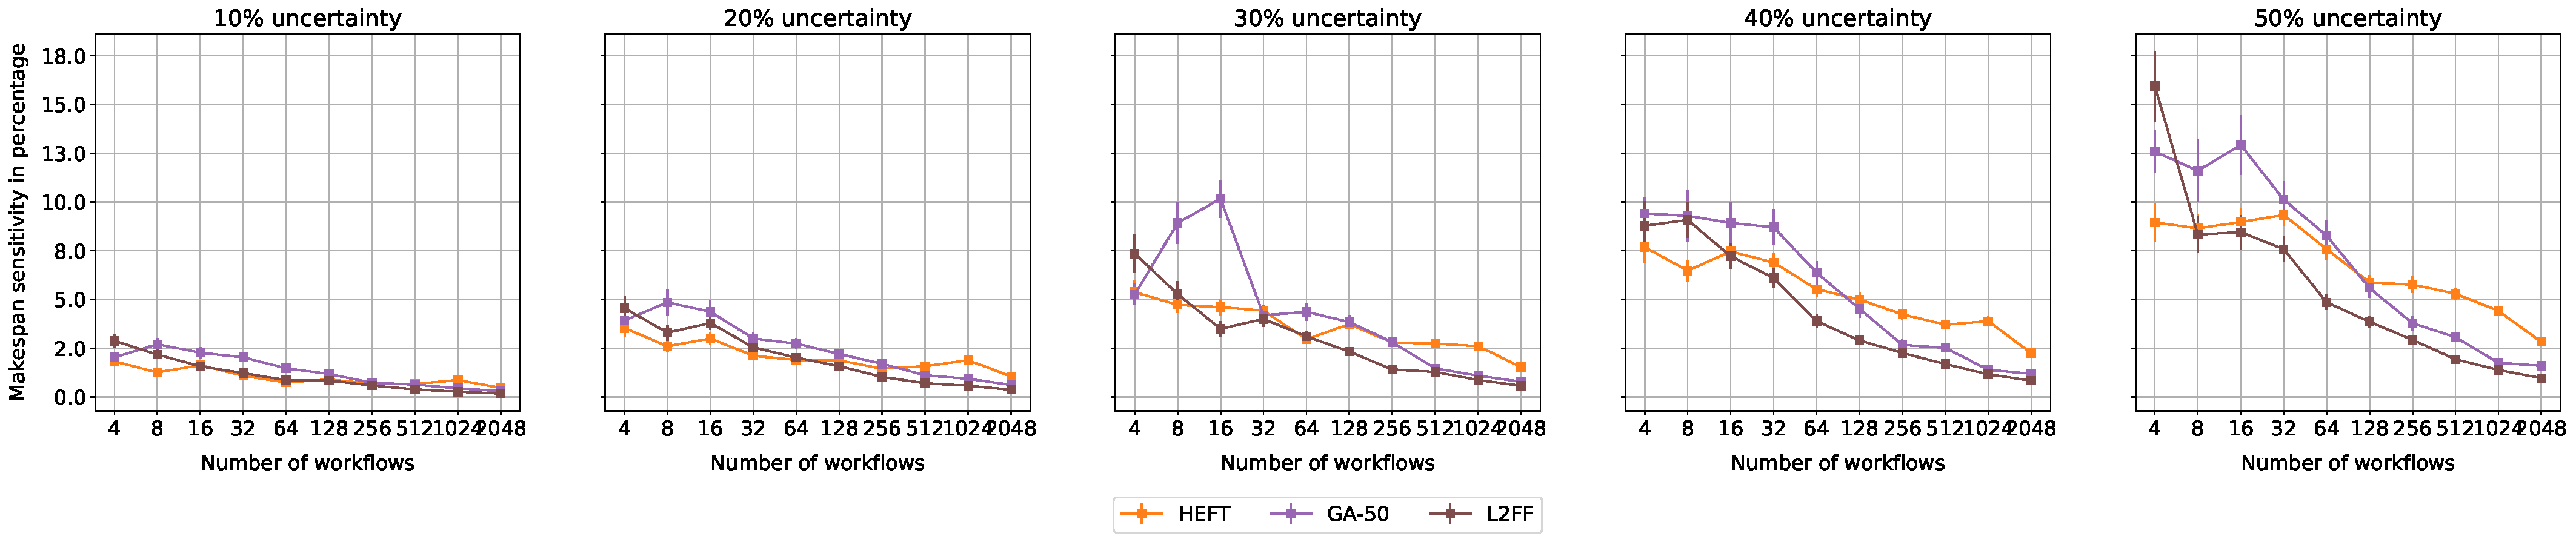
\includegraphics[width=.95\textwidth]{figures/campaign/InaccurStHeteroCampaigns_4StHeteroResourcesSens.pdf}
        \caption{}
        \label{fig:InaccurStHeteroCampaigns_4StHeteroResourcesSens}
    \end{subfigure}\\
    ~ 
    \begin{subfigure}[b]{0.95\textwidth}
        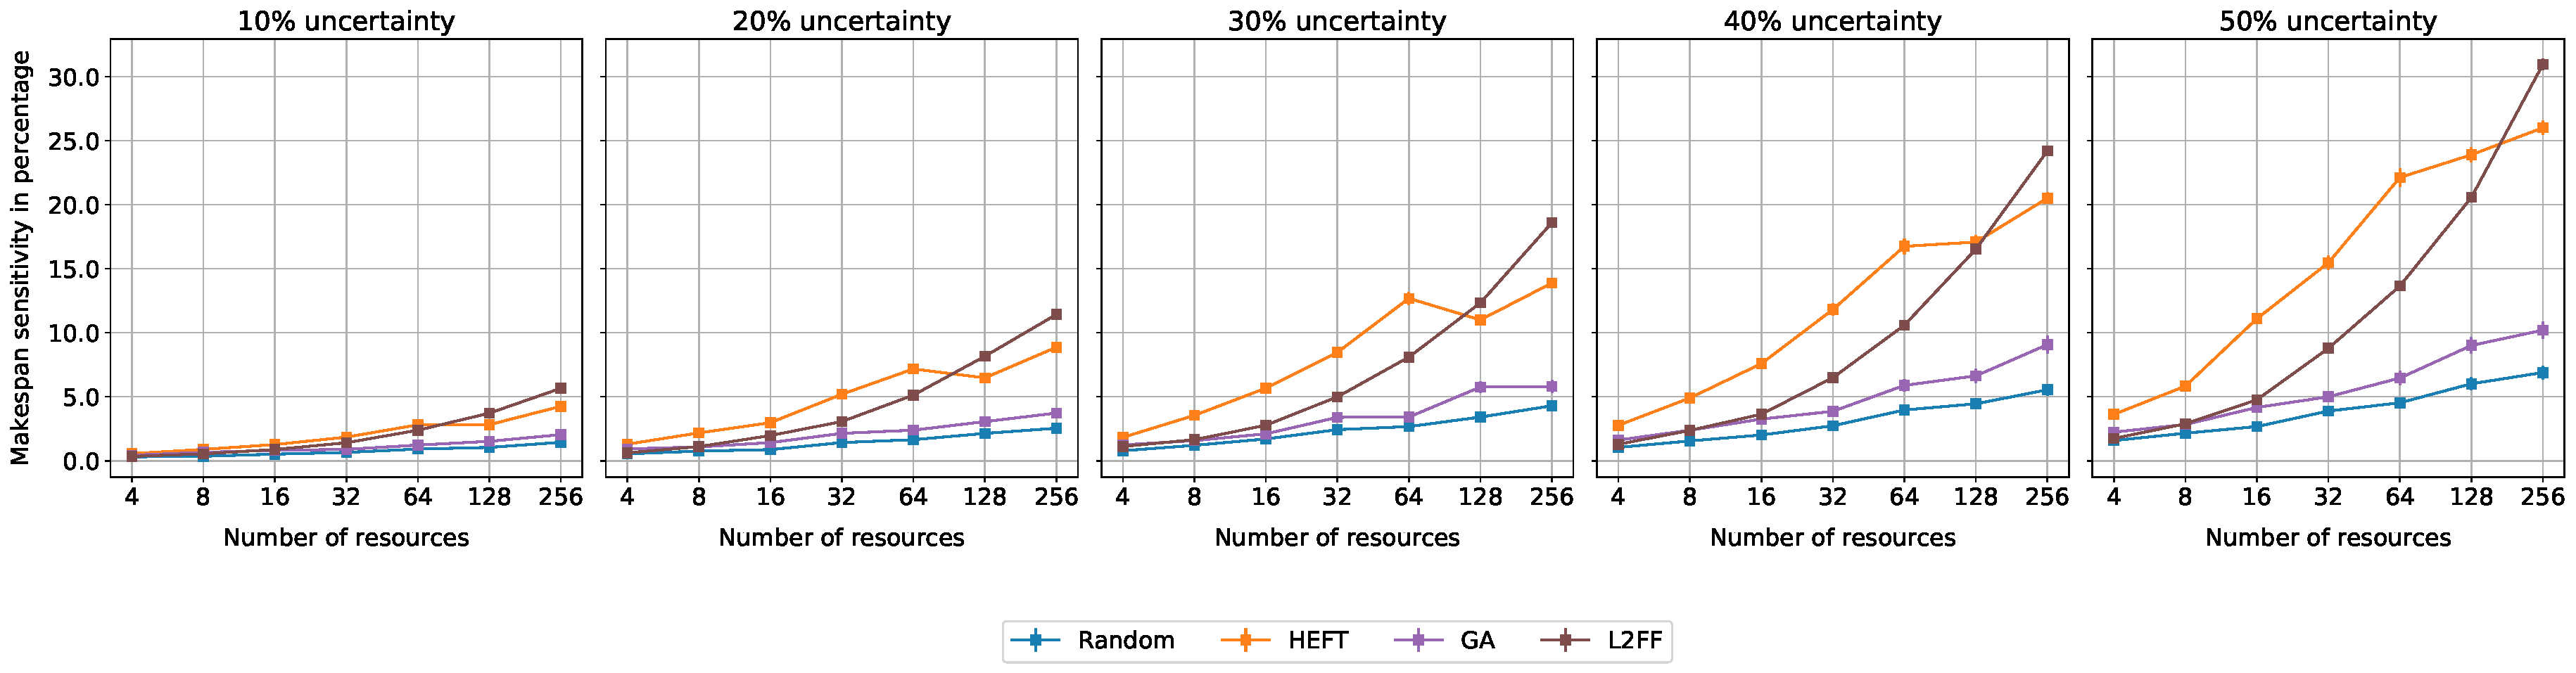
\includegraphics[width=0.95\textwidth]{figures/campaign/InaccurStHeteroResources_StHeteroCampaignsSens.pdf}
        \caption{}
        \label{fig:InaccurStHeteroResources_StHeteroCampaignsSens}
    \end{subfigure}
    \caption{~\ref{fig:InaccurStHeteroCampaigns_4StHeteroResourcesSens} Makespan sensitivity for different levels of uncertainty and different number of workflows on static resources;
    ~\ref{fig:InaccurStHeteroResources_StHeteroCampaignsSens} Makespan sensitivity for different levels of uncertainty and different number of resources on static resources.}
    \label{fig:inaccur_st}
\end{figure}

The ratio of number of workflows over the number of resources remains inverse proportional to the sensitivity.
In addition, specifically for HEFT the impact of uncertainty increases significantly as the number of resources increase, reaching 55~\%.
Since HEFT places one or two workflows on these resources, any change affects significantly its expected makespan.
This verifies our conclusion from experiment 2, that HEFT's strong assumptions about workflow length and resource availability makes it very sensitive to changes.

\begin{figure}[ht!]
    \centering
    \begin{subfigure}[b]{0.95\textwidth}
        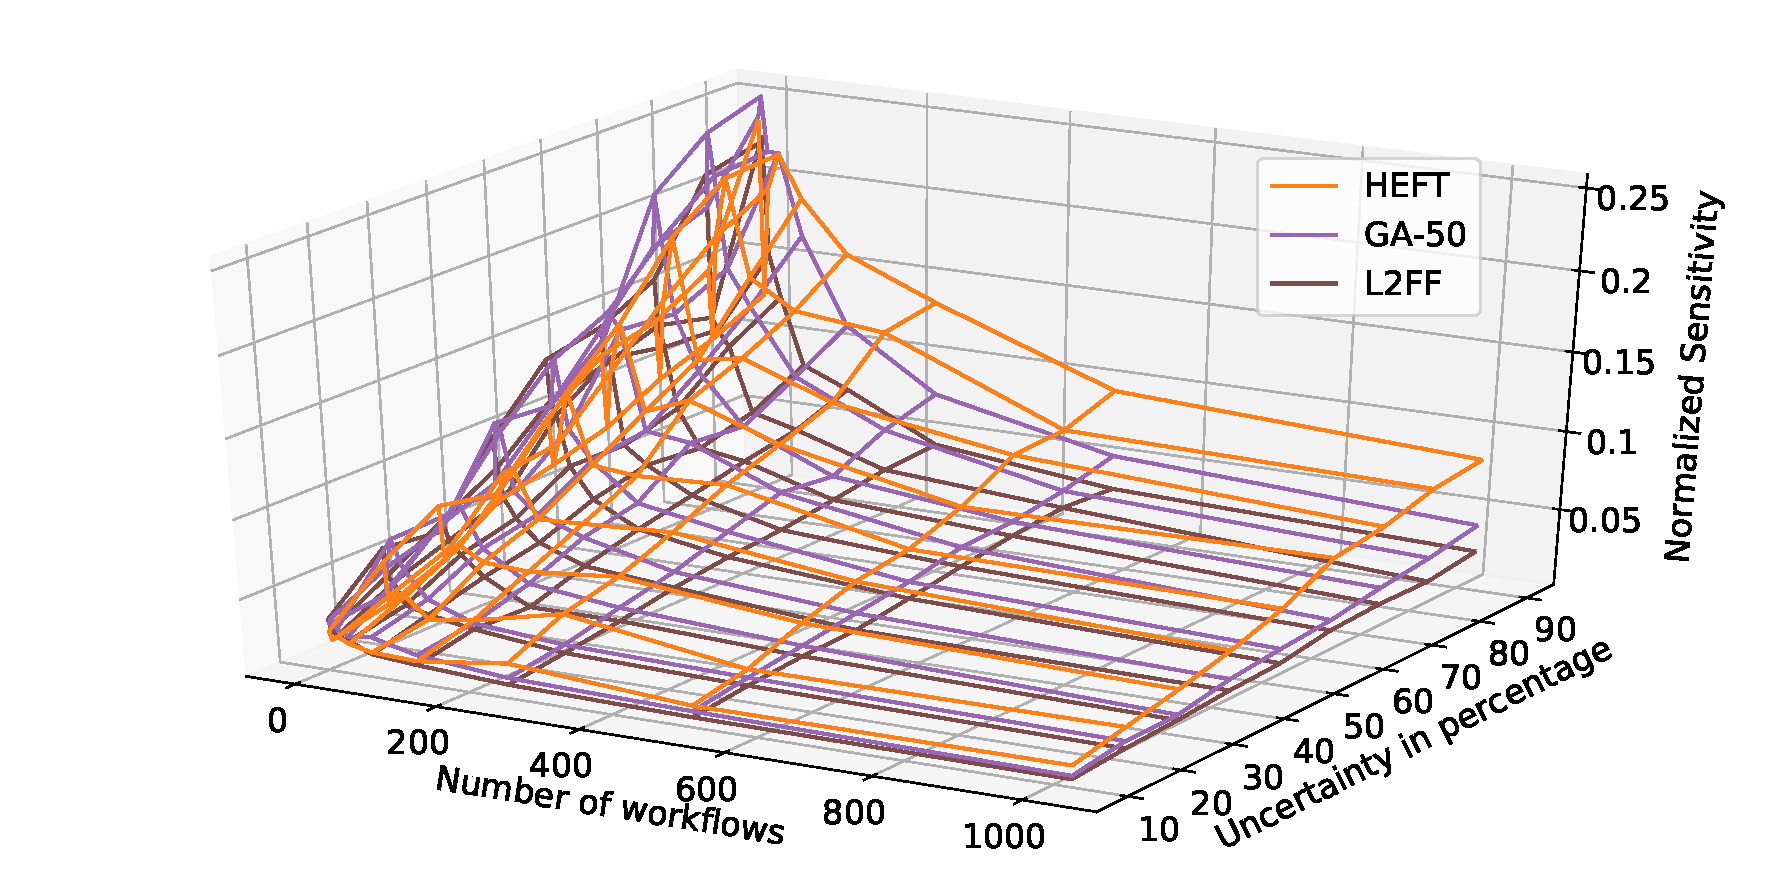
\includegraphics[width=.95\textwidth]{figures/campaign/InaccurStHeteroCampaigns_4DynHeteroResourcesSens.pdf}
        \caption{}
        \label{fig:InaccurStHeteroCampaigns_4DynHeteroResourcesSens}
    \end{subfigure}\\
    ~ 
    \begin{subfigure}[b]{0.95\textwidth}
        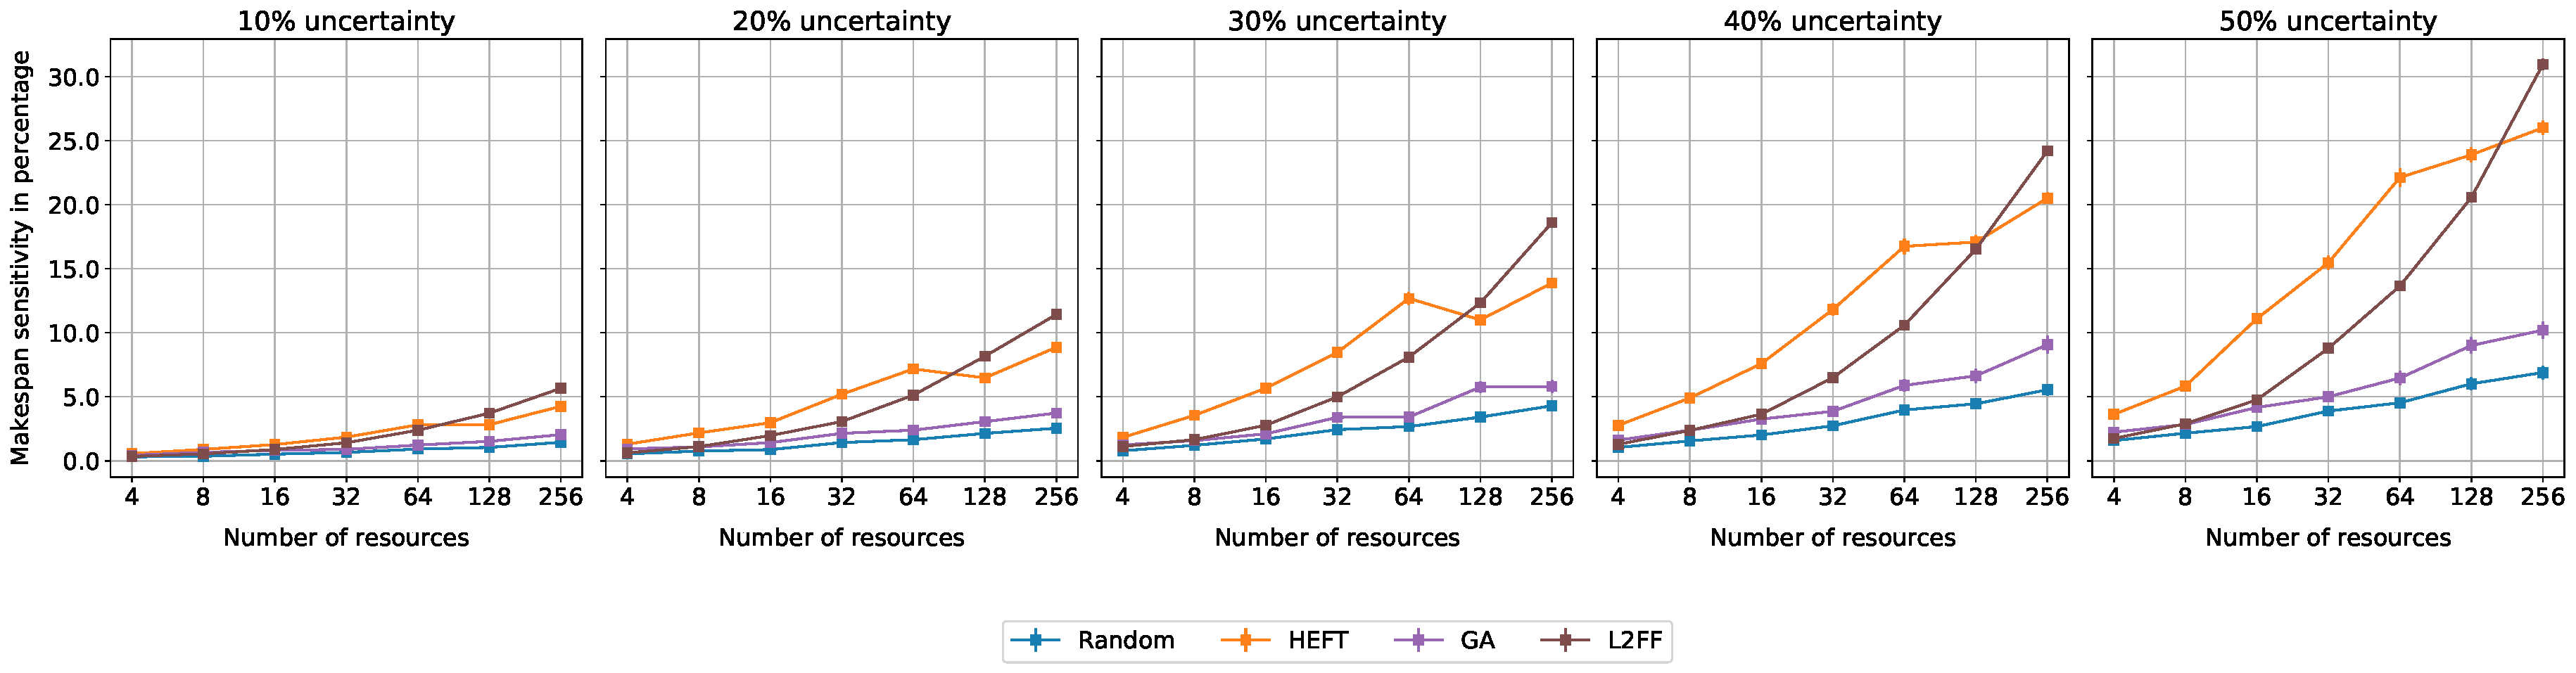
\includegraphics[width=0.95\textwidth]{figures/campaign/InaccurStHeteroResources_StHeteroCampaignsSens.pdf}
        \caption{}
        \label{fig:InaccurDynHeteroResources_StHeteroCampaignsSens}
    \end{subfigure}
    \caption{~\ref{fig:InaccurStHeteroCampaigns_4DynHeteroResourcesSens} Makespan sensitivity for different levels of uncertainty and different number of workflows on static resources;
    ~\ref{fig:InaccurDynHeteroResources_StHeteroCampaignsSens} Makespan sensitivity for different levels of uncertainty and different number of resources on static resources.}
    \label{fig:inaccur_dyn}
\end{figure}

Introducing resource dynamism increased further the sensitivity of the algorithms, as seen in figure~\ref{fig:inaccur_dyn}.
The observed increase was no more than the level shown in experiment 2.
This shows us that the overall sensitivity is the summation of independently measured sensitivity from different sources.

The results of our experiments show that algorithms which make significant assumptions about the workflow length and resource performance produce better makespan.
That is apparent from the fact that HEFT consistently produces the smaller makespan.
This is true also when resources are dynamic and the workflows runtime is uncertain even at 90~\%.
HEFT had a sensitivity of around 60~\% maximum which is not enough to affect the plan in such a way that another algorithm would be preferable.
Furthermore, knowledge of resource heterogeneity and availability is an important factor in differentiating the performance of the algorithms, as seen by the performance difference of L2FF compared to HEFT and GA.
Lastly, the ratio of the number of workflows over the number of resources affects the level of sensitivity of the algorithms.
The less number of workflows placed on resources higher the significance of a change either in the performance of the resources or the workflow runtime.
%\subsubsection{Time to calculate a plan}
%
%Based on experiments HEFT and L2FF will have the smallest overhead for calculating the makespan.
%This is due to their deterministic behavior.
%GA on the other hand is a non-deterministic algorithm and its runtime depends on its convergence rate.

\section{Conceptual Framework for Selecting Planning Algorithms}
\label{sec:cf_algo_sel}
Based on our analysis, we conclude that selecting algorithm 1 over algorithm 2 provides the better makespan in most cases. 
But due to the time scales at which the execution of a campaign runs, the computation complexity of the algorithm, as long as, it remains in the order of minutes is not significant.
In addition, selecting an algorithm that can encode resource availability is beneficial, since resources can become unavailable either due to performance dynamism, or due to unforeseen events